\documentclass[12pt]{article}

\usepackage[spanish]{babel}
\usepackage[none]{hyphenat}
\usepackage[left=1.5cm, right=1.5cm, top = 2cm, bottom=2.5cm]{geometry}
\usepackage{parskip}
\usepackage[export]{adjustbox}
\usepackage{enumitem}[shortlabels]
\usepackage{listings} 
\usepackage{color}
\usepackage{fancyhdr}
\usepackage{graphicx}
\usepackage{caption} 
% \usepackage{subcaption}
\usepackage{wrapfig}
% \usepackage{longtable}
% \usepackage{multirow, makecell}
% \usepackage{amsmath} 
\usepackage[hidelinks]{hyperref}
\usepackage{csquotes}
\usepackage{tocloft}
\usepackage{rotating}

\newcommand{\linejump}{\hfill \break}
\renewcommand{\thefootnote}{\fnsymbol{footnote}}
% \newcommand{\unit}[1]{\ensuremath{\, \mathrm{#1}}}

\definecolor{dkgreen}{rgb}{0,0.6,0}
\definecolor{gray}{rgb}{0.5,0.5,0.5}
\definecolor{mauve}{rgb}{0.58,0,0.82}
\lstset{
  language=Java,
  aboveskip=3mm,
  belowskip=3mm,
  showstringspaces=false,
  columns=flexible,
  basicstyle={\scriptsize\ttfamily},
  numbers=none,
  numberstyle=\tiny\color{gray},
  keywordstyle=\color{blue},
  commentstyle=\color{dkgreen},
  stringstyle=\color{mauve},
  breaklines=true,
  breakatwhitespace=true,
  tabsize=2
}

\sloppy
\setlength{\parindent}{0cm}
\setlength{\columnsep}{0.5cm}
\setlength{\cftbeforesecskip}{0.3cm}
\setlength{\cftbeforesubsecskip}{0.2cm}
\setlength{\cftbeforesubsubsecskip}{0.18cm}
\setlength{\cftbeforefigskip}{0.2cm}
\decimalpoint
\graphicspath{{img/}}

\hypersetup{colorlinks=true, urlcolor=blue, citecolor=blue, linkcolor=black}
\urlstyle{same}

\pagestyle{fancyplain}
\fancyhf{}
\fancyhead[L]{\scriptsize 
  Universidad Nacional Autónoma de México \\
  Programación Orientada a Objetos \\
  M.C. Leonardo Ledesma Dominguez
}
\fancyhead[R]{\thepage}

\begin{document}
  \begin{center}
    \linejump
    \LARGE \textbf{Proyecto Final. Primera entrega. Dominó}
  \end{center}

  \begin{flushright}
    \textbf{Integrantes} \\
    Acosta Porcayo Alan Omar 320206102 \\
    Gutiérrez Grimaldo Alejandro 320282098 \\ 
    Medina Villa Samuel 320249538 
  \end{flushright}

  \tableofcontents
  \newpage

  \section{Antecedentes históricos}
  El origen de este juego no es tan claro, ya que algunos historiadores y antropólogos fueron los griegos, también otros afirman que fueron los hebreos. Sin embargo, el juego actual del dominó parece que se inició en China, donde se jugaba hace 1.500 años de manera semejante a como se hace hoy. Se podría considerar como el primer dominó de la historia.
  
  La forma actual conocida en Europa y el mundo no aparece hasta el siglo XVIII, cuando lo introdujeron los italianos en este continente. Gracias a la enorme expansión de la cultura europea a través del mundo, llegó a diversos países y culturas.

  Inicialmente, las fichas se fabricaban mediante la unión de dos láminas de ébano en ambos lados de la ficha de hueso. Este método tenía la ventaja de prevenir posibles trampas al ocultar los puntos en la parte posterior de la ficha bajo ciertas condiciones de iluminación, además de crear un atractivo contraste entre los puntos blancos y el fondo negro, lo que permitía que el hueso fuera visible a través de los agujeros en el ébano.

  \section{Descripción}
  El objetivo principal del juego de dominó es ser el primer jugador en quedarse sin fichas en su mano. Para lograrlo, los jugadores deben emparejar las fichas que poseen con las que ya están en la mesa, asegurándose de que los números de los puntos coincidan. Esto implica tomar decisiones estratégicas sobre cuándo y cómo jugar sus fichas para maximizar sus posibilidades de quedarse sin fichas antes que sus oponentes. 

  \section{Definición de clases}
  \subsection{Clase \textit{Ficha}}
  Esta clase representa una ficha de dominó simple. 

  \subsubsection{Atributos}
  \begin{enumerate}
    \item \textit{caraIzq.} Variable privada de tipo \textit{int} con el valor de la parte izquierda de la ficha.
    \item \textit{caraDer.} Variable privada de tipo \textit{int} con el valor de la parte derecha de la ficha.
    \item \textit{suma.} Variable privada de tipo \textit{int} con la suma de ambas partes de la ficha, se calcula al momento de crear la ficha.
    \item \textit{mula.} Variable privada de tipo \textit{boolean} que indica si la ficha es una mula o no.
  \end{enumerate}

  \subsubsection{Métodos}
  \begin{enumerate}
    \item \textit{Ficha(int caraIzq, int caraDer).} Método constructor que recibe dos enteros que representan los valores de las caras de la ficha. Calcula la suma y determina si la ficha es una mula.
    \item \textit{getCaraIzq().} Método público que retorna el valor de la cara izquierda de la ficha.
    \item \textit{getCaraDer().} Método público que retorna el valor de la cara derecha de la ficha.
    \item \textit{getSuma().} Método público que retorna el valor de la suma de la ficha.
    \item \textit{esMula().} Método público que retorna un booleano que indica si la ficha es una mula o no. 
    \item \textit{girar().} Método público que intercambia los valores de las caras de la ficha.
    \item \textit{toString().} Método público (sobreescritura) que retorna una cadena con formato del valor de las caras de la ficha.
  \end{enumerate}

  \subsection{Clase Abstracta \textit{Jugador}}
  Esta clase representa a un jugador de dominó, ya sea persona o bot.

  \subsubsection{Atributos}
  \begin{enumerate}
    \item \textit{nombre.} Variable protegida de tipo \textit{String} con el nombre del jugador.
    \item \textit{fichas.} Variable protegida de tipo \textit{ArrayList$<$Ficha$>$} con las fichas del jugador.
    \item \textit{puedeJugar.} Variable protegida de tipo \textit{boolean} que indica si el jugador tiene una ficha que pueda jugar.
  \end{enumerate}

  \subsubsection{Métodos}
  \begin{enumerate}
    \item \textit{getNombre().} Método público que retorna el nombre del jugador.
    \item \textit{getFichas().} Método público que retorna las fichas del jugador.
    \item \textit{getFicha(int i).} Método público que retorna la ficha en la posición \textit{i} del jugador.

    \item \textit{agregarFicha(Ficha ficha).} Método público que agrega una ficha a las fichas del jugador.
    \item \textit{puedeJugar().} Método público que retorna un booleano que indica si el jugador puede jugar.
    \item \textit{puedeJugar(ArrayList$<$Ficha$>$ mesa).} Método público (sobrecarga) que comprueba si dentro de las fichas del jugador hay alguna que pueda jugarse en la mesa actual y actualiza el valor de \textit{puedeJugar}.
    \item \textit{robar(ArrayList$<$Ficha$>$ pozo).} Método público que sustrae una ficha del pozo y la agrega a las fichas del jugador.
    \item \textit{primerTurno(ArrayList$<$Ficha$>$ mesa).} Método público que realiza el primer turno del jugador.
    \item \textit{turno(ArrayList$<$Ficha$>$ mesa).} Método final y público que realiza el turno del jugador. Se divide en pasos que son métodos abstractos y concretos que son implementados en las subclases \textit{Persona} y \textit{Bot}.
    \item \textit{buscarFicha(ArrayList<Ficha> mesa).} Método abstracto que devuelve la instrucción de la ficha y su orientación en la mesa.
    \item \textit{validarFicha(ArrayList<Ficha> mesa, int indice, char orientacion).} Método privado que es un paso del método \textit{turno} que valida si la ficha que se quiere jugar es válida.
    \item \textit{jugarFicha(ArrayList<Ficha> mesa, int indice, char orientacion).} Método privado que es un paso del método \textit{turno} que juega la ficha en la mesa.  
  \end{enumerate}

  \subsection{Clase \textit{Persona}}
  Esta clase representa a un jugador controlado por el usuario.

  \subsubsection{Métodos}
  \begin{enumerate}
    \item \textit{Humano(String nombre).} Método constructor que recibe el nombre del jugador.
    \item \textit{buscarFicha(ArrayList<Ficha> mesaActual).} Método protegido (sobreescritura) que le pide al usuario que ingrese el índice de la ficha que quiere jugar y la orientación en la que la quiere jugar. 
  \end{enumerate}

  \subsection{Clase \textit{Bot}}
  Esta clase representa a un jugador controlado por la computadora.

  \subsubsection{Métodos}
  \begin{enumerate}
    \item \textit{Bot(String nombre).} Método constructor que recibe el nombre del jugador.
    \item \textit{turno(ArrayList$<$Ficha$>$ mesaActual).} Método protected (sobreescritura) que busca una ficha para jugar en la mesa actual.
    \item \textit{evaluarFicha(Ficha ficha, ArrayList<Ficha> mesa).} Método privado que calcula las posibilidades de una de las fichas del bot.
    \item \textit{contarPosibilidades(Ficha ficha, ArrayList<Ficha> mesa).} Método privado que cuenta las posibilidades de una de las fichas del bot.
    \item \textit{elegirFichaGenerica(ArrayList<Ficha> mesa).} Método privado que solo se utiliza en caso de que los métodos \textit{evaluarFicha} y \textit{contarPosibilidades} no encuentren una ficha para jugar.
  \end{enumerate}

  \subsection{Clase \textit{Modelo}} 
  Esta clase representa la mesa de juego. 

  \subsubsection{Atributos}
  \begin{enumerate}
    \item \textit{mesa.} Variable privada de tipo \textit{ArrayList$<$Ficha$>$} con las fichas de la mesa.
    \item \textit{pozo.} Variable privada de tipo \textit{ArrayList$<$Ficha$>$} con las fichas sobrantes del juego.
    \item \textit{jugadores.} Variable privada de tipo \textit{List$<$Jugador$>$} con los jugadores del juego. Inicialmente contiene un objeto de tipo \textit{Humano} y dos de tipo \textit{Bot}.
    \item \textit{turno.} Variable privada de tipo \textit{int} que lleva la cuenta de los turnos.
  \end{enumerate}

  \subsubsection{Métodos}
  \begin{enumerate}
    \item \textit{Modelo(String nombre).} Primer método constructor (sobrecarga) que recibe el nombre del jugador y crea un objeto de tipo \textit{Persona} con ese nombre y un objeto de tipo \textit{Bot}, reparte las fichas y decide quien empieza el juego.
    \item \textit{Modelo().} Segundo método constructor (sobrecarga) que crea dos objetos de tipo \textit{Bot}, reparte las fichas y decide quien empieza el juego.
    \item \textit{Modelo(Configuracion conf).} Tercer método constructor (sobrecarga) que recibe un objeto de tipo \textit{Configuracion} y copia los jugadores y el pozo de la configuración.
    \item \textit{getMesa().} Método público que retorna las fichas de la mesa.
    \item \textit{getPozo().} Método público que retorna las fichas del pozo.
    \item \textit{getTamanioPozo().} Método publico que retorna el tamaño del pozo.
    \item \textit{getJugadores().} Método público que retorna los jugadores del juego.
    \item \textit{getJugador(int i)} Método público que retorna un objeto de tipo \textit{Jugador} en la posición \textit{i} de la lista de jugadores.
    \item \textit{getTurno().} Método público que retorna el turno actual.
    \item \textit{repartir().} Método privado que crea los objetos de tipo \textit{Ficha}, los agrega al pozo, los mezcla y los reparte entre los jugadores.
    \item \textit{decidirPrimerTurno().} Método privado que determina quien empieza el juego buscando quien tiene la mula mas alta y si no hay mula, quien tiene la ficha con la suma mas alta. En caso de que el primer turno sea del jugador en la posición 1 de la lista de jugadores se cambia el orden de los jugadores.
    \item \textit{cambioDeTurno().} Método público que cambia el orden de los jugadores en la lista.
  \end{enumerate}

  \subsection{Clase \textit{Historial}}
  Esta clase permite guardar y cargar un historial de partidas en un archivo de texto.

  \subsubsection{Métodos}
  \begin{enumerate}
    \item \textit{getHistorial().} Método público y estático que retorna un objeto de tipo \textit{ArrayList$<$Partida$>$} con las partidas guardadas en el archivo de texto.
    \item \textit{guardarResultado(String nombre, int turno).} Método público y estático que recibe el nombre del ganador y el número de turnos que duró la partida y lo guarda en el archivo de texto junto con la fecha actual.
  \end{enumerate}

  \subsection{Clase \textit{Partida}}
  Esta clase representa una partida guardada en el historial.

  \subsubsection{Atributos}
  \begin{enumerate}
    \item \textit{nombre.} Variable privada de tipo \textit{String} con el nombre del ganador.
    \item \textit{turno.} Variable privada de tipo \textit{int} con el número de turnos que duró la partida.
    \item \textit{fecha.} Variable privada de tipo \textit{String} con la fecha en la que se jugó la partida.
  \end{enumerate}

  \subsubsection{Métodos}
  \begin{enumerate}
    \item \textit{getNombre().} Método público que retorna el nombre del ganador.
    \item \textit{getTurno().} Método público que retorna el número de turnos que duró la partida.
    \item \textit{getFecha().} Método público que retorna la fecha en la que se jugó la partida.
  \end{enumerate}

  \subsection{Clase \textit{Configuracion}}
  Esta clase permite guardar y cargar una configuración de una partida en un archivo de texto debido a la serialización y deserialización.

  \subsubsection{Atributos}
  \begin{enumerate}
    \item \textit{pozo.} Variable privada de tipo \textit{ArrayList$<$Ficha$>$} con las fichas del pozo.
    \item \textit{jugadores.} Variable privada de tipo \textit{ArrayList$<$Jugador$>$} con los jugadores de la partida.
    \item \textit{listaArchivos.} Variable privada, estática y trasndental de tipo \textit{ArrayList$<$String$>$} con los nombres de los archivos de texto en la carpeta \textit{configuraciones}.
  \end{enumerate}

  \subsubsection{Métodos}
  \begin{enumerate}
    \item \textit{Configuracion(String nombreArchivo).} Primer método constructor (sobrecarga) que recibe el nombre del archivo de texto y carga la configuración de la partida guardada en el archivo.
    \item \textit{Configuracion(ArrayList<Ficha> pozo, ArrayList<Jugador> jugadores).} Segundo método constructor (sobrecarga) privado que recibe el pozo y los jugadores de una partida.
    \item \textit{getPozo().} Método público que retorna las fichas del pozo.
    \item \textit{getJugadores().} Método público que retorna los jugadores de la partida.
    \item \textit{getListaArchivos().} Método público y estático que retorna un objeto de tipo \textit{ArrayList$<$String$>$} con los nombres de los archivos de texto en la carpeta \textit{configuraciones}.
    \item \textit{guardarConfiguracion(String nombreArchivo, ArrayList<Ficha> pozo, ArrayList<Jugador> jugadores).} Método público y estático que recibe el nombre del archivo de texto, el pozo y los jugadores de una partida y guarda la configuración en el archivo utilizando el método constructor privado.
  \end{enumerate}

  \subsection{Clase \textit{Musica}}
  Esta clase permite reproducir clips de audio.

  \subsubsection{Atributos}
  \begin{enumerate}
    \item \textit{musica.} Variable privada y estática de tipo \textit{Clip} que representa el clip de audio.
  \end{enumerate}

  \subsubsection{Métodos}
  \begin{enumerate}
    \item \textit{reiniciarMusica()} Método público que reinicia el clip de audio.
    \item \textit{musicaFinal().} Método público que reproduce el clip de audio de victoria.
  \end{enumerate}

  \subsection{Clase \textit{Controlador}}
  Esta clase permite controlar el flujo del programa.

  \subsubsection{Atributos}
  \begin{enumerate}
    \item \textit{sc.} Variable privada y estática de tipo \textit{Scanner} que permite leer las entradas del usuario.
    \item \textit{modelo.} Variable privada y estática de tipo \textit{Modelo} que representa la mesa de juego.
    \item \textit{musica.} Variable privada y estática de tipo \textit{Musica} que permite reproducir clips de audio.
    \item \textit{ESPERA.} Variable privada, estática y final de tipo \textit{int} que representa el tiempo de espera entre turnos.
    \item \textit{opcion.} Variable privada y estática de tipo \textit{int} que representa la opción seleccionada por el usuario en el menú.
  \end{enumerate}

  \subsubsection{Métodos}
  \begin{enumerate}
    \item \textit{main(String[] args).} Método público y estático que inicia el programa y controla el flujo del mismo.
    \item \textit{esperar(int tiempo).} Método privado y estático que recibe un entero que representa el tiempo de espera en milisegundos.
    \item \textit{guardarConfiguracion().} Método privado y estático que guarda le pregunta al usuario si desea guardar la configuración de la partida actual y la guarda en caso de que la respuesta sea afirmativa.
    \item \textit{continuarJuego().} Método privado y estático que evalua las condiciones para continuar el juego de acuerdo a las fichas de los jugadores y el pozo.
    \item \textit{decidirGanador().} Método privado y estático que determina quien es el ganador de la partida.
  \end{enumerate}

  \subsection{Clase interna \textit{HiloTurno}}
  Esta clase permite realizar el turno de un jugador en un hilo diferente al principal.

  \subsubsection{Atributos}
  \begin{enumerate}
    \item \textit{jugador.} Variable privada de tipo \textit{Jugador} que representa al jugador que va a realizar su turno.
    \item \textit{mesa.} Variable privada de tipo \textit{ArrayList$<$Ficha$>$} que representa las fichas de la mesa.
    \item \textit{turno.} Variable privada de tipo \textit{int} que representa el turno actual.
    \item \textit{tamanioPozo.} Variable privada de tipo \textit{int} que representa el tamaño del pozo.
  \end{enumerate}

  \subsubsection{Métodos}
  \begin{enumerate}
    \item \textit{HiloTurno(Jugador jugador, ArrayList<Ficha> mesa, int turno, int tamanioPozo).} Método constructor que recibe el jugador que va a realizar su turno, las fichas de la mesa, el turno actual y el tamaño del pozo.
    \item \textit{run().} Método público (sobreescritura) que realiza el turno del jugador.
  \end{enumerate}

  \subsection{Clase \textit{Vista}}
  Esta clase permite imprimir en la terminal.

  \subsubsection{Métodos}
  \begin{enumerate}
    \item \textit{limpiarPantalla().} Método público y estático que limpia la terminal.
    \item \textit{continuar().} Método público y estático que le pide al usuario que presione enter para continuar.
    \item \textit{pedirNombre().} Método público y estático que le pide al usuario que ingrese su nombre.
    \item \textit{mostrarMenu().} Método público y estático que imprime el menú de opciones.
    \item \textit{mostrarPozo(int pozo).} Método público y estático que imprime el número de fichas en el pozo.
    \item \textit{mostrarTurno(String nombre).} Método público y estático que imprime el nombre del jugador que tiene el turno. 
    \item \textit{mostrarMesa(ArrayList<Ficha> mesa).} Método público y estático que imprime las fichas de la mesa.
    \item \textit{mostrarFichas(ArrayList<Ficha> fichas).} Método público y estático que imprime las fichas de un jugador.
    \item \textit{mostrarGanador(String nombre).} Método público y estático que imprime el nombre del ganador.
    \item \textit{mostrarEmpate().} Método público y estático que imprime un mensaje de empate.
    \item \textit{mostrarHistorial(ArrayList<Partida> historial).} Método público y estático que imprime el historial de partidas.
    \item \textit{mostrarArchivos(ArrayList<String> archivos).} Método público y estático que imprime los nombres de los archivos de texto en la carpeta \textit{configuraciones}. 
  \end{enumerate}

  \section{Definición de objetos}
  \begin{itemize}
    \item \textit{ArrayList$<$Ficha$>$.} Colección de objetos de tipo \textit{Ficha}. Se crea para representar las fichas de la mesa, las fichas del pozo y las fichas de los jugadores.
    \item \textit{ArrayList$<$Jugador$>$.} Colección de objetos de tipo \textit{Jugador}. Se crea para representar los jugadores de la partida.
    \item \textit{ArrayList$<$Partida$>$.} Colección de objetos de tipo \textit{Partida}. Se crea para representar las partidas guardadas en el historial.
    \item \textit{ArrayList$<$String$>$.} Colección de objetos de tipo \textit{String}. Se crea para representar los nombres de los archivos de texto en la carpeta \textit{configuraciones}.
    \item \textit{Scanner.} Objeto que permite leer las entradas del usuario.
    \item \textit{Clip.} Objeto que permite reproducir clips de audio.
    \item \textit{ProcessBuilder.} Objeto que permite ejecutar comandos en la terminal.
    \item \textit{Thread.} Objeto que permite crear hilos.
    \item \textit{ObjectInputStream.} Objeto que permite deserializar objetos.
    \item \textit{ObjectOutputStream.} Objeto que permite serializar objetos.
    \item \textit{File.} Objeto que permite crear archivos.
    \item \textit{FileReader.} Objeto que permite leer archivos.
    \item \textit{BufferedReader.} Objeto que permite leer archivos.
    \item \textit{FileWriter.} Objeto que permite escribir archivos.
    \item \textit{BufferedWriter.} Objeto que permite escribir archivos.
    \item \textit{Date.} Objeto que permite obtener la fecha actual.
  \end{itemize}

  \section{Algoritmo}
  Se comienza creando un objeto \textit{Scanner} llamado \textit{sc} para leer las entradas del usuario y un objeto \textit{Clip} llamado \textit{musica} para reproducir los clips de audio. Para reproducir un clip se hace dentro de un bloque \textit{try-catch} para evitar que el programa se detenga en caso de que no se encuentre el archivo de audio.

  \begin{lstlisting}
Scanner sc = new Scanner(System.in);
Clip musica = null;

try {
  musica = AudioSystem.getClip();
  musica.open(AudioSystem.getAudioInputStream(Domino.class.getResource("/recursos/MoonlightSonata.wav")));
  musica.loop(Clip.LOOP_CONTINUOUSLY); 
} catch (Exception e) {
  e.printStackTrace();
}
  \end{lstlisting}

  Luego, se imprime el menú con las opciones de juego para que el usuario pueda seleccionar jugador vs bot o bot vs bot. Se lee la entrada del usuario y se crea un objeto de tipo \textit{Mesa} llamado \textit{mesa} con el tipo de juego seleccionado por el usuario.

  \begin{lstlisting}
System.out.println("%%%%%%%%%%%%%%% Bienvenido a Domino %%%%%%%%%%%%%%%");
System.out.println("Escoga el modo de juego:");
System.out.println("1. Jugador vs Bot");
System.out.println("2. Bot vs Bot");
System.out.print("$ ");
int tipoJuego = sc.nextInt();
Mesa mesa = new Mesa(tipoJuego);
  \end{lstlisting}

  Dentro de un ciclo \textit{while} con la condición de repetición de que los jugadores tengan fichas y el pozo no este vacío, se limpia la terminal usando una un bloque \textit{try-catch} y un objeto \textit{ProcessBuilder}.

  \begin{lstlisting}
try {
  new ProcessBuilder("cmd", "/c", "cls").inheritIO().start().waitFor();
} catch (Exception e) {
  e.printStackTrace();
}
  \end{lstlisting}

  Posteriormente, se imprime las fichas de la mesa, el número de fichas en el pozo y se anuncia el turno del jugador en la posición 0 de la lista de jugadores e imprime sus fichas. 

  \begin{lstlisting}
System.out.println("\n\nMesa actual:");
mesa.imprimir();
System.out.println("\nNumero de fichas en el Pozo: " + mesa.getPozo().size());

System.out.println("\n%%%%% Turno de " + mesa.getJugadores().get(0).getNombre() + " %%%%%");
mesa.imprimir(mesa.getJugadores().get(0).getFichas());
  \end{lstlisting}
 
  El siguiente bloque de código corresponde al turno de los jugadores. Si la mesa esta vacia quiere decir que es el primer turno, en ese caso se llama al método \textit{primerTurno} y se continua con el flujo del programa. Para los turnos siguientes primero se comprueba si el jugador puede jugar una ficha realiza su turno con el método \textit{turno}. En caso de que no pueda jugar y no haya fichas en el pozo se imprime un mensaje diciendo que el jugador con el turno actual pasa de turno, y si hay fichas en el pozo roba una, se vuelve a imprimir sus fichas y se pasa de turno. 

  \begin{lstlisting}
if (mesa.getMesa().isEmpty())
  mesa.getJugadores().get(0).primerTurno(mesa.getMesa());
else {
  if (mesa.getJugadores().get(0).puedeJugar(mesa.getMesa())) 
    mesa.getJugadores().get(0).turno(mesa.getMesa());
  else { 
    if (mesa.getPozo().isEmpty()) { 
      System.out.println("No puedes jugar y no hay fichas en el pozo, pasas tu turno");

      try {
        Thread.sleep(3000);
      } catch (InterruptedException e) {
        e.printStackTrace();
      }
    } else {
      if (mesa.getJugadores().get(0) instanceof Humano)
        System.out.println("Necesitas robar una ficha");

      try {
        Thread.sleep(3000);
      } catch (InterruptedException e) {
        e.printStackTrace();
      }

      System.out.println(mesa.getJugadores().get(0).getNombre() + " roba 1 ficha y pasa su turno");
      mesa.getJugadores().get(0).robar(mesa.getPozo());
      mesa.imprimir(mesa.getJugadores().get(0).getFichas());

      try {
        Thread.sleep(3000);
      } catch (InterruptedException e) {
        e.printStackTrace();
      }
    }
  }
}
  \end{lstlisting}

  Al salir del ciclo \textit{while}, dentro de un bloque \textit{try-catch} se para la reproducción del clip de audio y se inicia otro clip de audio con la música de victoria. 

  \begin{lstlisting}
try {
  if (musica != null)
    musica.stop();
  
  musica = AudioSystem.getClip();
  musica.open(AudioSystem.getAudioInputStream(Domino.class.getResource("/recursos/Victoria.wav")));
  musica.start();
} catch (Exception e) {
  e.printStackTrace();
}        
  \end{lstlisting}

  Para terminar se decide el ganador. Si un jugador se queda sin fichas se imprime un mensaje diciendo que gano pero si el pozo se vacía se busca quien tiene la suma más alta y se imprime un mensaje diciendo que gano o si hay empate.

  \begin{lstlisting}
if (!mesa.getJugadores().get(0).puedeJugar() && 
      !mesa.getJugadores().get(1).puedeJugar() &&
      mesa.getPozo().isEmpty() ) {
  int suma1 = 0, suma2 = 0;
  System.out.println("Se acabaron las fichas");

  for (int i = 0; i < mesa.getJugadores().get(0).getCantidadFichas(); i++)
    suma1 += mesa.getJugadores().get(0).getFicha(i).getSuma();
  for (int i = 0; i < mesa.getJugadores().get(1).getCantidadFichas(); i++)
    suma2 += mesa.getJugadores().get(1).getFicha(i).getSuma();
  
  if (suma1 < suma2)
    System.out.println("El ganador es " + mesa.getJugadores().get(0).getNombre());
  else if (suma1 > suma2)
    System.out.println("El ganador es " + mesa.getJugadores().get(1).getNombre());
  else
    System.out.println("Empate");
} else 
  System.out.println("\n%%%%%%%%%% El ganador es " + mesa.getJugadores().get(0).getNombre() + " %%%%%%%%%%");
  \end{lstlisting}

  \section{Herencia de clases}
  La herencia de clases se utilizó principalmente en las clases \textit{Jugador}, \textit{Persona} y \textit{Bot}. La clase \textit{Jugador} es una clase abstracta que tiene los atributos y métodos que comparten los jugadores de la partida. La clase \textit{Persona} hereda de la clase \textit{Jugador} y tiene los métodos que permiten al usuario jugar su turno. La clase \textit{Bot} hereda de la clase \textit{Jugador} y tiene los métodos que permiten al bot jugar su turno.

  Otra herencia de clases se encuentra en la clase interna \textit{HiloTurno} que extiende de la clase \textit{Thread} y se sobreescribe el método \textit{run} para que el jugador realice su turno.

  \section{Implementación de interfaces}
  La implementación de interfaces se utilizó en la clases \textit{Configuracion}, \textit{Ficha} y \textit{Jugador} para la serialización y deserialización de objetos. La clase \textit{Configuracion} implementa la interfaz \textit{Serializable} para poder serializar los \textit{ArrayList} de jugadores y fichas del pozo de una partida en un archivo txt y poder cargarla posteriormente si el usuario lo desea.

  \section{Manejo de excepciones}
  Para el manejo de excepciones se utilizó principalmente los bloques \textit{try-catch} para evitar que el programa se detenga en caso de que ocurra un error como en el ejemplo siguiente que involucra el uso de hilos:

  \begin{lstlisting}
 try {
  Thread.sleep(tiempo);
} catch (InterruptedException e) {
  e.printStackTrace();
}
  \end{lstlisting}

  En otras ocasiones se utilizó el bloque \textit{try-catch-with-resources} para cerrar los recursos utilizados en el programa como en el ejemplo siguiente:

  \begin{lstlisting}
try (ObjectInputStream ois = new ObjectInputStream(new FileInputStream("configuraciones/" + nombreArchivo))) {
  Configuracion conf = (Configuracion) ois.readObject();
  this.pozo = conf.getPozo();
  this.jugadores = conf.getJugadores();
} catch (Exception e) {
  System.out.println("Error al cargar la configuracion");
}
  \end{lstlisting}

  Además, implementamos excepciones propias para manejar los errores de entrada del usuario como en el siguiente ejemplo:

  \begin{lstlisting}
try {
  System.out.println("Donde la quieres jugar? (i o d)");
  System.out.print("$ ");
  orientacion = sc.next().charAt(0);
  if (orientacion != 'i' && orientacion != 'd') 
    throw new OrientacionInvalidaException("Orientacion no valida. Debe ser 'i' o 'd'.");
} catch (OrientacionInvalidaException e) {
  System.out.println(e.getMessage() + "\n");
}
  \end{lstlisting}

  Las excepciones propias que creamos son: 

  \begin{lstlisting}
package domino;

/**
 * Excepcion lanzada cuando se recibe una respuesta invalida.
 */
class RespuestaInvalidaException extends Exception {
  /**
    * Constructor de la excepcion.
    * @param mensaje Mensaje que describe la naturaleza de la respuesta invalida.
    */
  public RespuestaInvalidaException(String mensaje) {
    super(mensaje);
  }
}

/**
 * Excepcion lanzada cuando se recibe un indice de ficha invalido.
 */
class IndiceFichaInvalidoException extends Exception {
  /**
    * Constructor de la excepcion.
    * @param mensaje Mensaje que describe la naturaleza del indice de ficha invalido.
    */
  public IndiceFichaInvalidoException(String mensaje) {
    super(mensaje);
  }
}

/**
 * Excepcion lanzada cuando se recibe una orientacion invalida.
 */
class OrientacionInvalidaException extends Exception {
  /**
    * Constructor de la excepcion.
    * @param mensaje Mensaje que describe la naturaleza de la orientacion invalida.
    */
  public OrientacionInvalidaException(String mensaje) {
    super(mensaje);
  }
}
  \end{lstlisting}

  \section{Manejo de archivos y serialización}
  En cuanto a manejo de archivos se utilizó la lectura/escritura de un historial de partidas en un archivo de texto con la clase Historial. Las entradas del archivo se guardan con ayuda de una instancia de la clase \textit{Partida} que tiene los atributos del nombre del ganador, el numero de turnos y la fecha de la partida.
  
  \begin{figure}[h!]
    \centering
    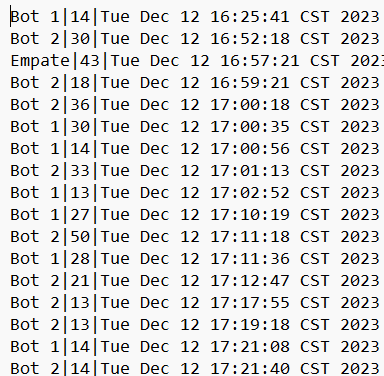
\includegraphics[width=0.4\textwidth]{historial.png}
    \caption{Ejemplo de un historial de partidas}
  \end{figure}
 
  Para la serialización se utilizó la clase Configuración para guardar el \textit{ArrayList} de jugadores y fichas del pozo de una partida en un archivo txt y poder cargarla posteriormente si el usuario lo desea. Esto se logró implementando la interfaz \textit{Serializable} y los métodos \textit{guardarConfiguracion} y \textit{cargarConfiguracion}.

  \section{Programación concurrente}
  La programación concurrente se utilizó para el turno de un jugador en la clase \textit{Controlador}, se creó una clase interna llamada \textit{HiloTurno} que extiende de la clase \textit{Thread} y se sobreescribió el método \textit{run} para que el jugador realice su turno. Evitando de esta manera que un jugador pueda jugar mientras el otro esta jugando.
  
  \begin{lstlisting}
/**
* Representa un hilo para manejar el turno de un jugador en un juego de domino.
*/
public static class HiloTurno extends Thread {
  private Jugador jugador;
  private ArrayList<Ficha> mesa;
  private int turno;
  private int tamanioPozo;

  /**
    * Construye un nuevo objeto HiloTurno.
    * 
    * @param jugador     el jugador asociado con el hilo
    * @param mesa        la lista de fichas de domino en la mesa
    * @param turno       el numero de turno actual
    * @param tamanioPozo el tamanio del monton de robo
    */
  public HiloTurno(Jugador jugador, ArrayList<Ficha> mesa, int turno, int tamanioPozo) {
    this.jugador = jugador;
    this.mesa = mesa;
    this.turno = turno;
    this.tamanioPozo = tamanioPozo;
  }

  /**
    * Ejecuta la logica del turno del jugador.
    */
  @Override
  public void run() {
    if (turno == 1) {
      jugador.primerTurno(mesa);
      esperar(ESPERA);
    } else {
      if (jugador.puedeJugar(mesa)) {
        if (jugador instanceof Bot)
          esperar(ESPERA);
        jugador.turno(mesa);
      } else {
        if (tamanioPozo == 0)
          System.out.println("No puedes jugar, pasas el turno");
        else {
          esperar(ESPERA);
          System.out.println("No puedes jugar, robas una ficha");
          esperar(ESPERA);
          jugador.robar(modelo.getPozo());
          Vista.mostrarFichas(jugador.getFichas());
        }
      }
    }
  }
}
  \end{lstlisting}
  \section{Patrones de diseño}
  Los patrones de diseño que aplicamos fueron dos: el patrón Modelo-Vista-Controlador \textit{MVC} y el patrón de comportamiento \textit{Template Method}. \textit{MVC} se utilizó en la estructura general del código, dividiéndolo en 3 secciones importantes como su nombre lo indica y utilizando otras clases ya sea para hacer conjunción de objetos o utilizar sus metodos dentro de las clases principales. 
  
  \textit{Template Method} se utilizó en la clase \textit{Jugador} para crear un método \textit{final} con el algoritmo del turno de un jugador, y separando el algoritmo en pasos en forma de métodos abstractos y concretos. De manera que las subclases \textit{Persona} y \textit{Bot} puedan implementar los métodos abstractos de manera diferente y así cambiar el algoritmo del turno de un jugador dependiendo del tipo de jugador.

  \section{Conclusiones}
  En este proyecto de implementación de un juego de dominó en Java, se han abordado de manera integral aspectos clave de la programación orientada a objetos y la interacción con el usuario. La estructura del diseño se fundamenta en la encapsulación de fichas, jugadores y la mesa en clases independientes, fomentando así una organización eficiente y facilitando el mantenimiento del código.

  La simulación del juego sigue meticulosamente las reglas auténticas del dominó, destacándose por su atención al detalle en la determinación de la jugabilidad de las fichas conforme a las reglas del juego. La gestión de situaciones como el robo de fichas y el cambio de turno se ejecuta de manera efectiva, evidenciando una comprensión profunda de las dinámicas del dominó. Esta capacidad se ha logrado mediante la aplicación de herencia y la implementación de métodos abstractos en las clases de jugadores.

  Además, la implementación aborda de manera proactiva la gestión de excepciones, asegurando que el juego sea robusto y confiable en diversas circunstancias. Este enfoque en la robustez del código no solo garantiza una experiencia de juego fluida, sino que también demuestra un compromiso con las mejores prácticas de programación.

  La realización de este proyecto no solo ha permitido aplicar las habilidades adquiridas durante el curso, sino que también ha fomentado la investigación y el trabajo colectivo. Este tipo de esfuerzo colaborativo promueve el desarrollo integral de habilidades, consolidando el aprendizaje teórico en un contexto práctico y realista.

  \section{Referencias}
  De Tenis De Huelva, R. C. R. (s. f.). \textit{Dominó} | \url{https://rcrtenishuelva1889.com/page/9/domino#:~:text=El%20domin%C3%B3%20surgi%C3%B3%20hace%20mil,los%20italianos%20por%20todas%20partes} \\

  Familia Vintage. (2018, June 5). \textit{Como Jugar Al Domino, Reglas del Dominó} [Video]. YouTube. \url{https://www.youtube.com/watch?v=-hbARCT1qow} \\

  Historia, C., $\&$ Historia, C. (2023, 22 abril). \textit{La historia del dominó, es una de las más interesantes que existe Read more}. CurioSfera Historia. \url{https://curiosfera-historia.com/historia-del-domino-origen-inventor/} \\

  \textit{Java Platform SE 8}. (2023). Oracle.com. \url{https://docs.oracle.com/javase/8/docs/api/} \\

  JUEGOS CON HISTORIA: \textit{El Dominó} | Lekotek. (s. f.). \url{https://www.lekotek.org.ar/juegos-con-historia-el-domino/} \\

  Solano, J. (2017, 20 enero). \textit{Manual de prácticas de Programación Orientada a Objetos}. Laboratorio de Computación Salas A y B. \url{http://lcp02.fi-b.unam.mx/} 

  \newpage
  \section{Apéndice}
  \subsection{Diagramas UML de clases}
  \begin{figure}[h!]
    \centering
    \begin{minipage}[l]{0.45\textwidth}
      \centering
      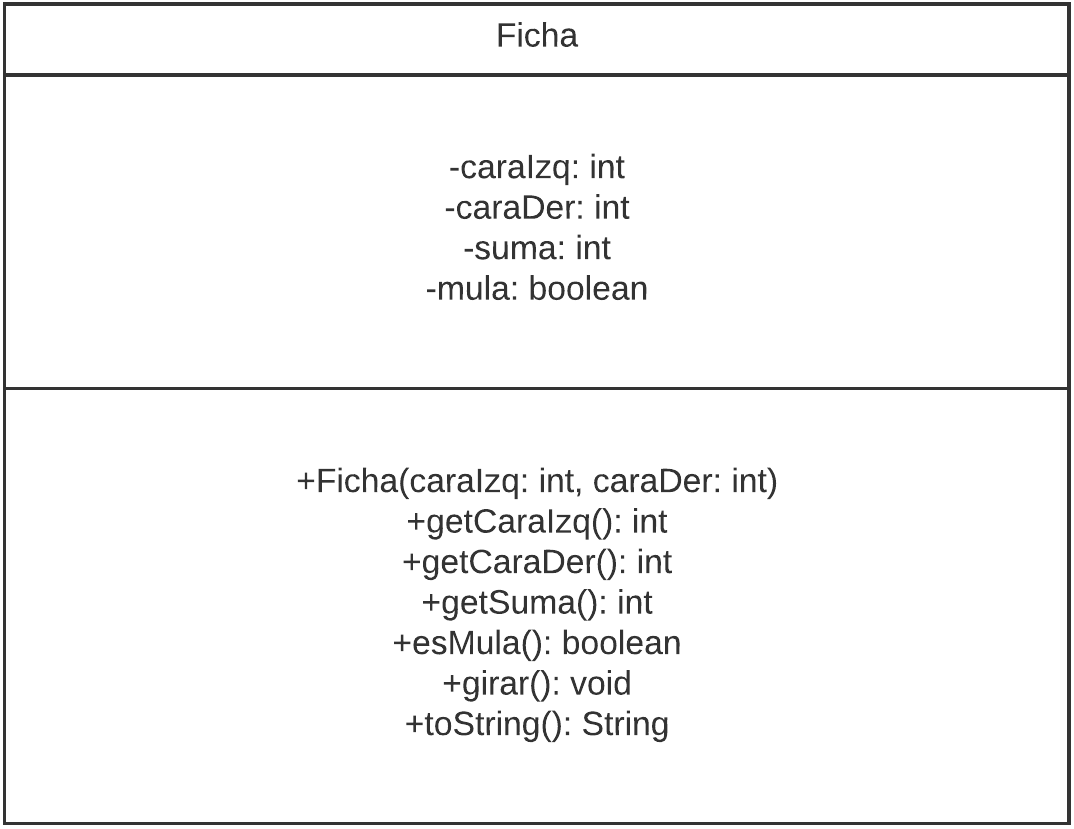
\includegraphics[height=5.5cm]{uml1.png}
      \caption{UML de clase \textit{Ficha}}
    \end{minipage}
    \begin{minipage}[r]{0.45\textwidth}
      \centering
      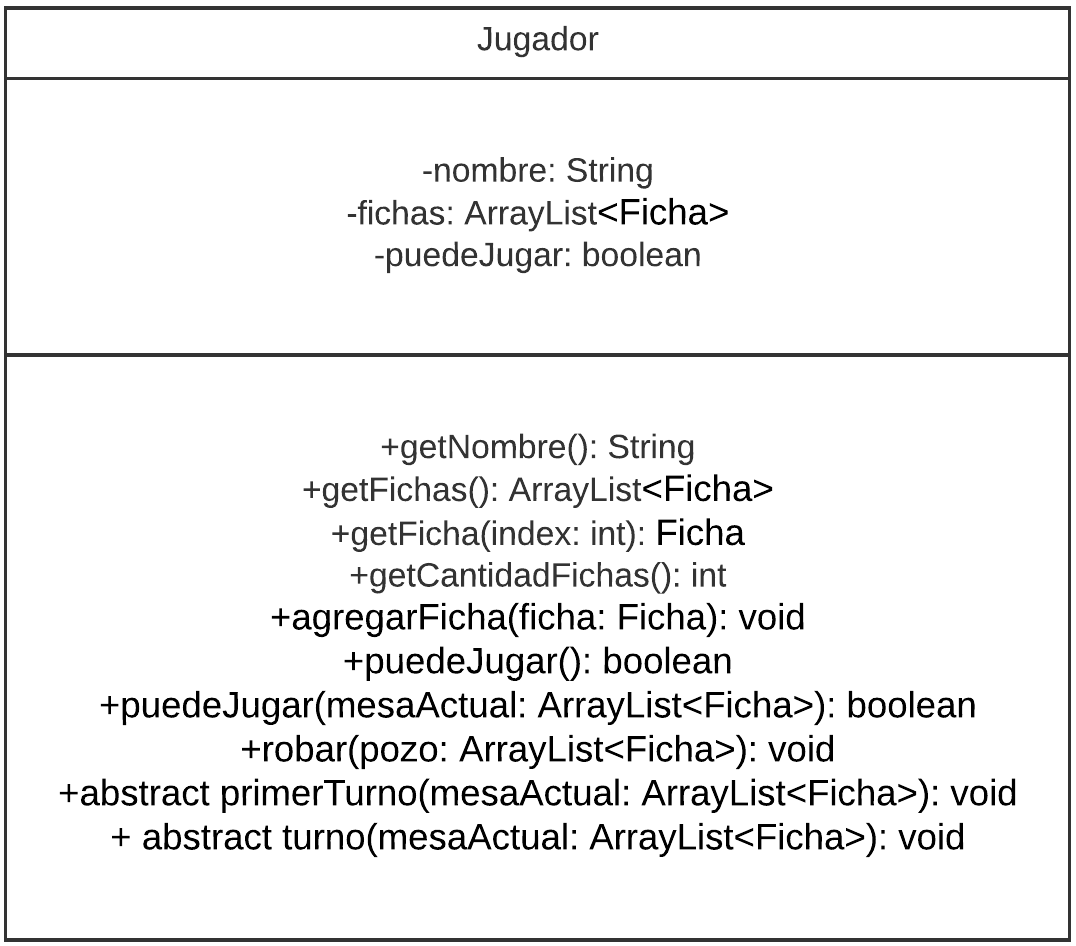
\includegraphics[height=5.5cm]{uml2.png}
      \caption{UML de clase \textit{Jugador}}
    \end{minipage}
  \end{figure}

  \begin{figure}[h!]
    \centering
    \begin{minipage}[l]{0.45\textwidth}
      \centering
      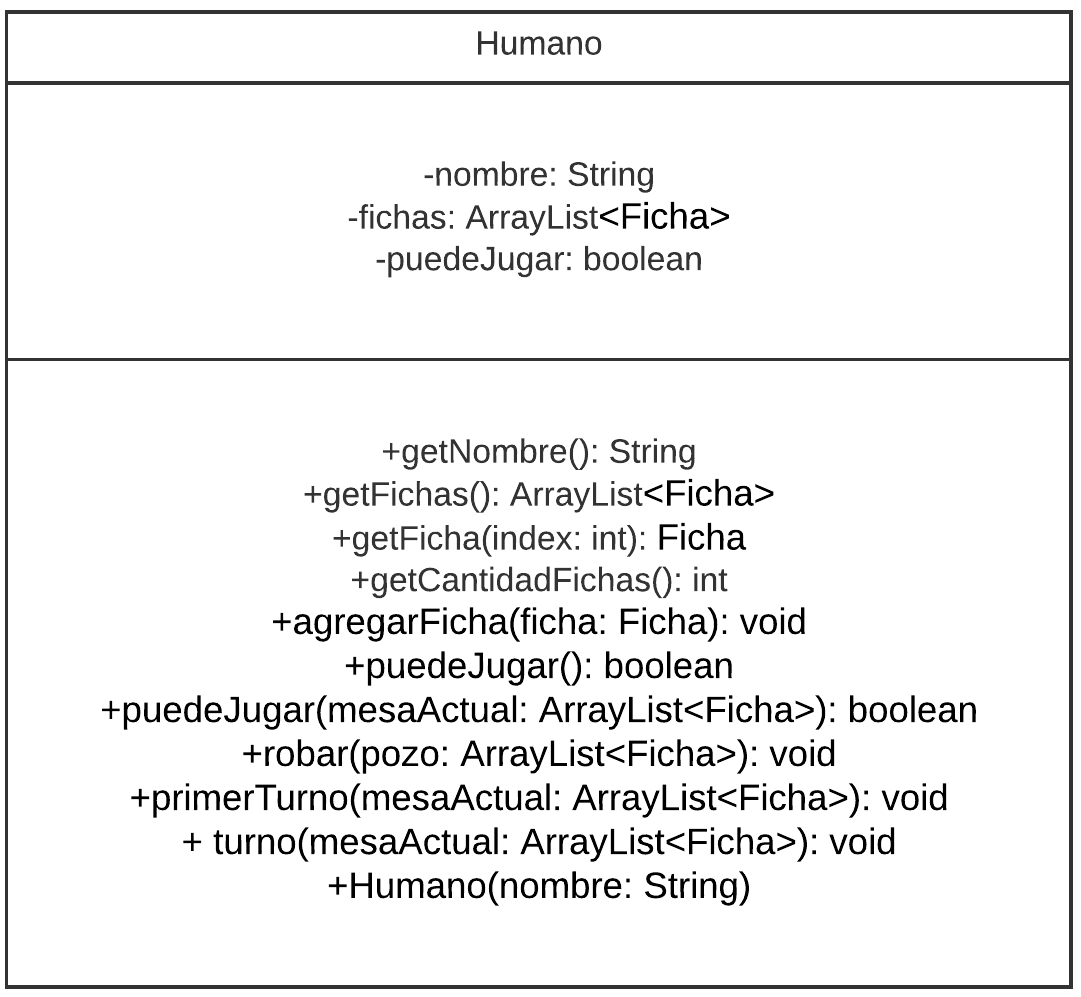
\includegraphics[height=5.5cm]{uml3.png}
      \caption{UML de clase \textit{Humano}}
    \end{minipage}
    \begin{minipage}[r]{0.45\textwidth}
      \centering
      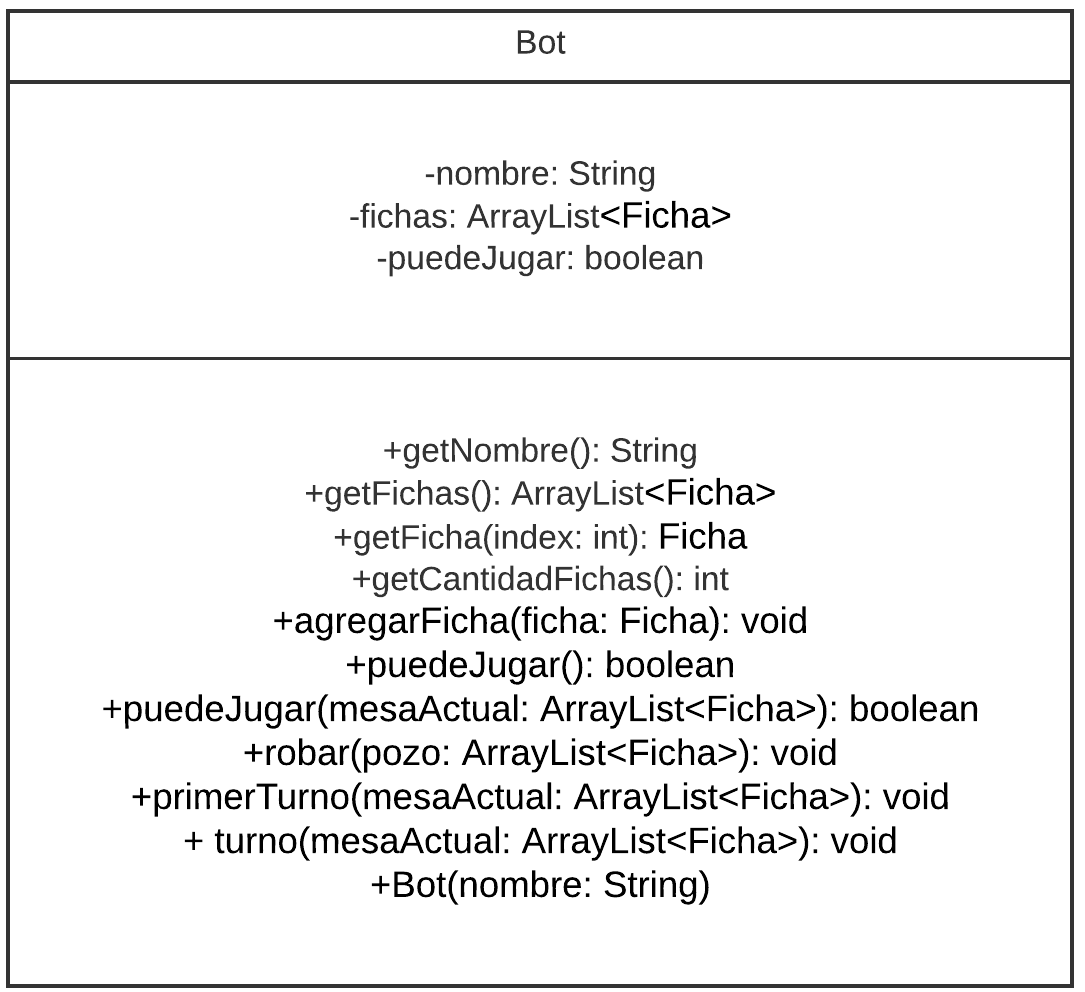
\includegraphics[height=5.5cm]{uml4.png}
      \caption{UML de clase \textit{Bot}}
    \end{minipage}
  \end{figure}

  \begin{figure}[h!]
    \centering
    \begin{minipage}[l]{0.45\textwidth}
      \centering
      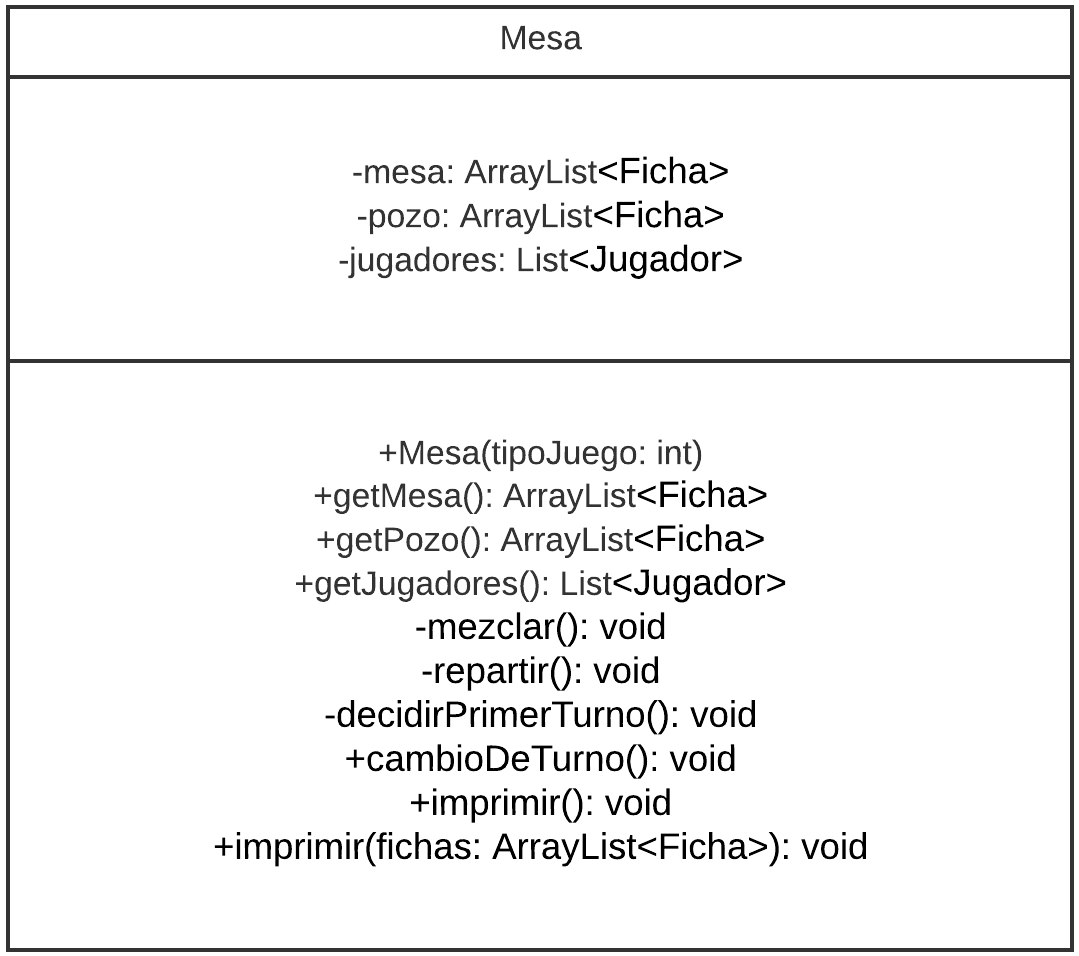
\includegraphics[height=5.5cm]{uml5.png}
      \caption{UML de clase \textit{Mesa}}
    \end{minipage}
    \begin{minipage}[r]{0.45\textwidth}
      \centering
      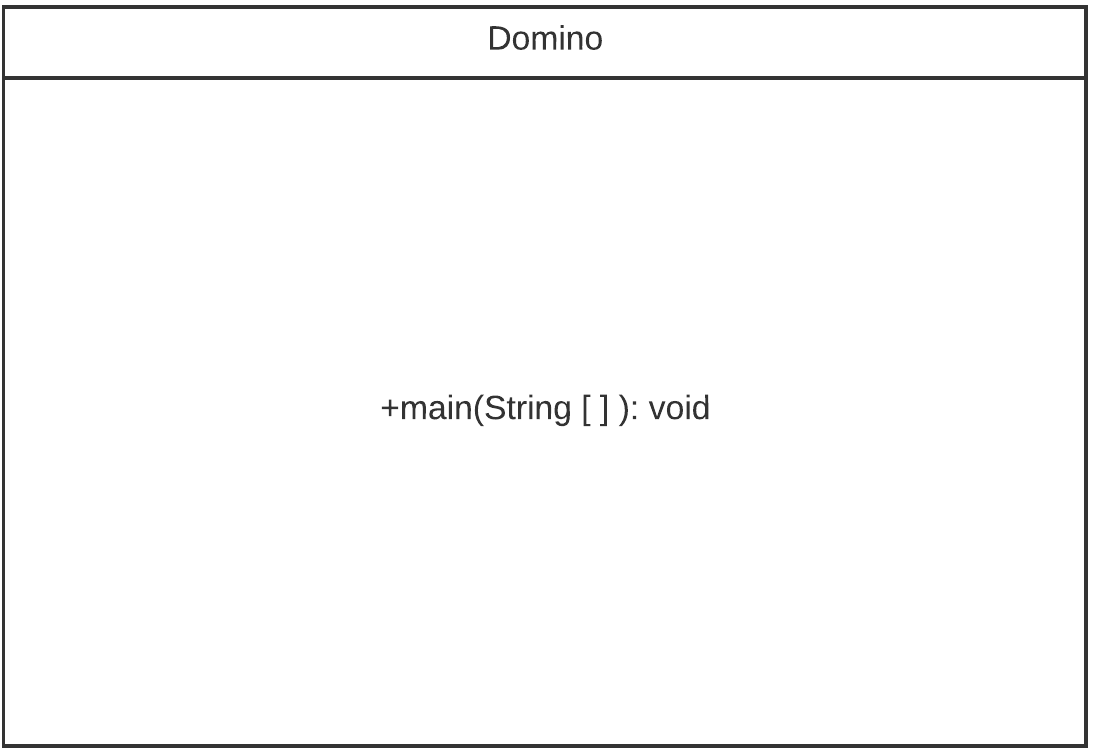
\includegraphics[height=5.5cm]{uml6.png}
      \caption{UML de clase \textit{Domino}} 
    \end{minipage}
  \end{figure}

  \linejump

  \subsection{Diagramas UML de objetos}
  \begin{figure}[h!]
    \centering
    \begin{minipage}[l]{0.45\textwidth}
      \centering
      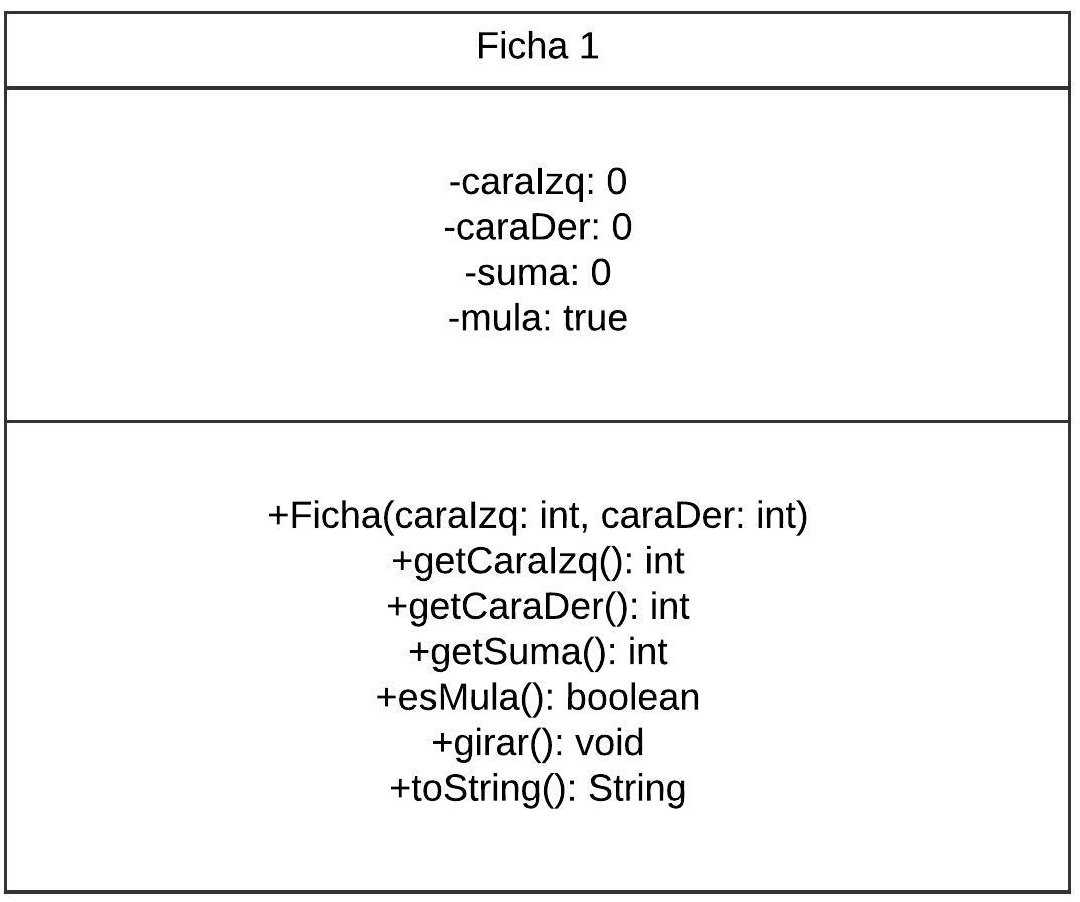
\includegraphics[height=6cm]{umlo1.png}
      \caption{UML de objeto \textit{Ficha1}}
    \end{minipage}
    \begin{minipage}[r]{0.45\textwidth}
      \centering
      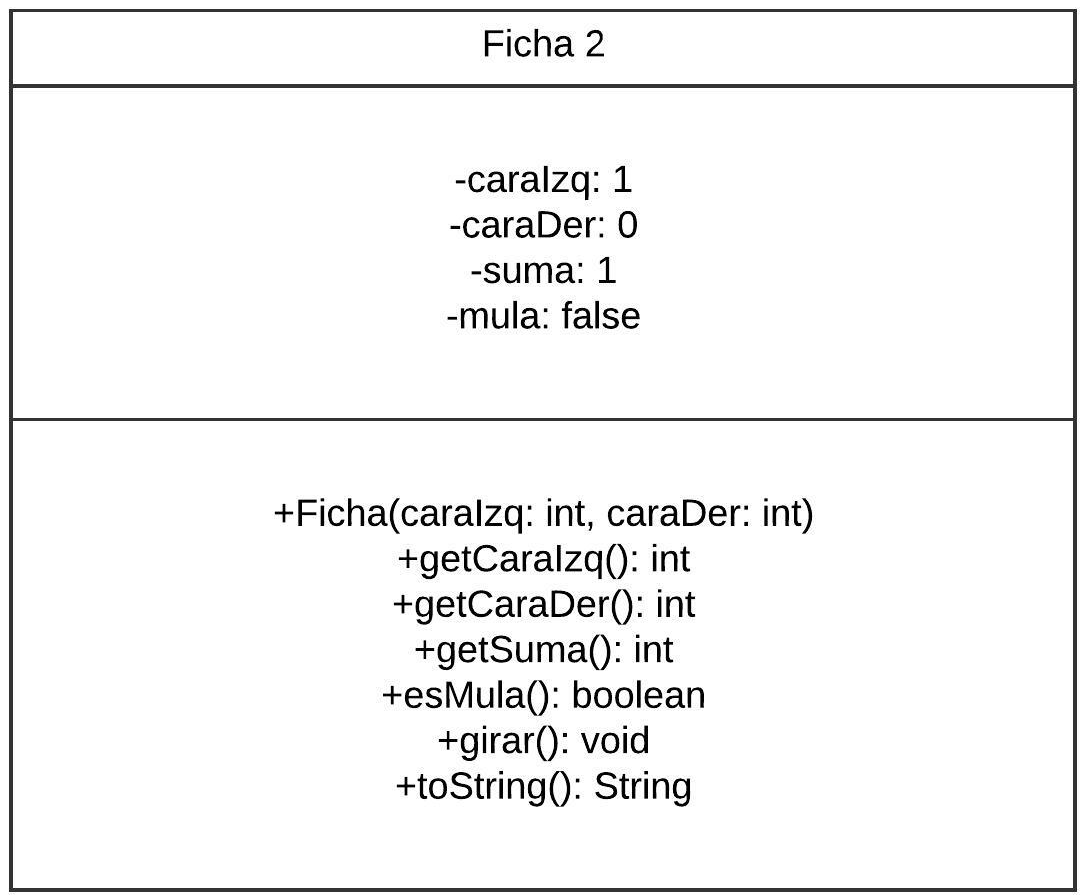
\includegraphics[height=6cm]{umlo2.png}
      \caption{UML de objeto \textit{Ficha2}}
    \end{minipage}
  \end{figure}

  \begin{figure}[h!]
    \centering
    \begin{minipage}[l]{0.45\textwidth}
      \centering
      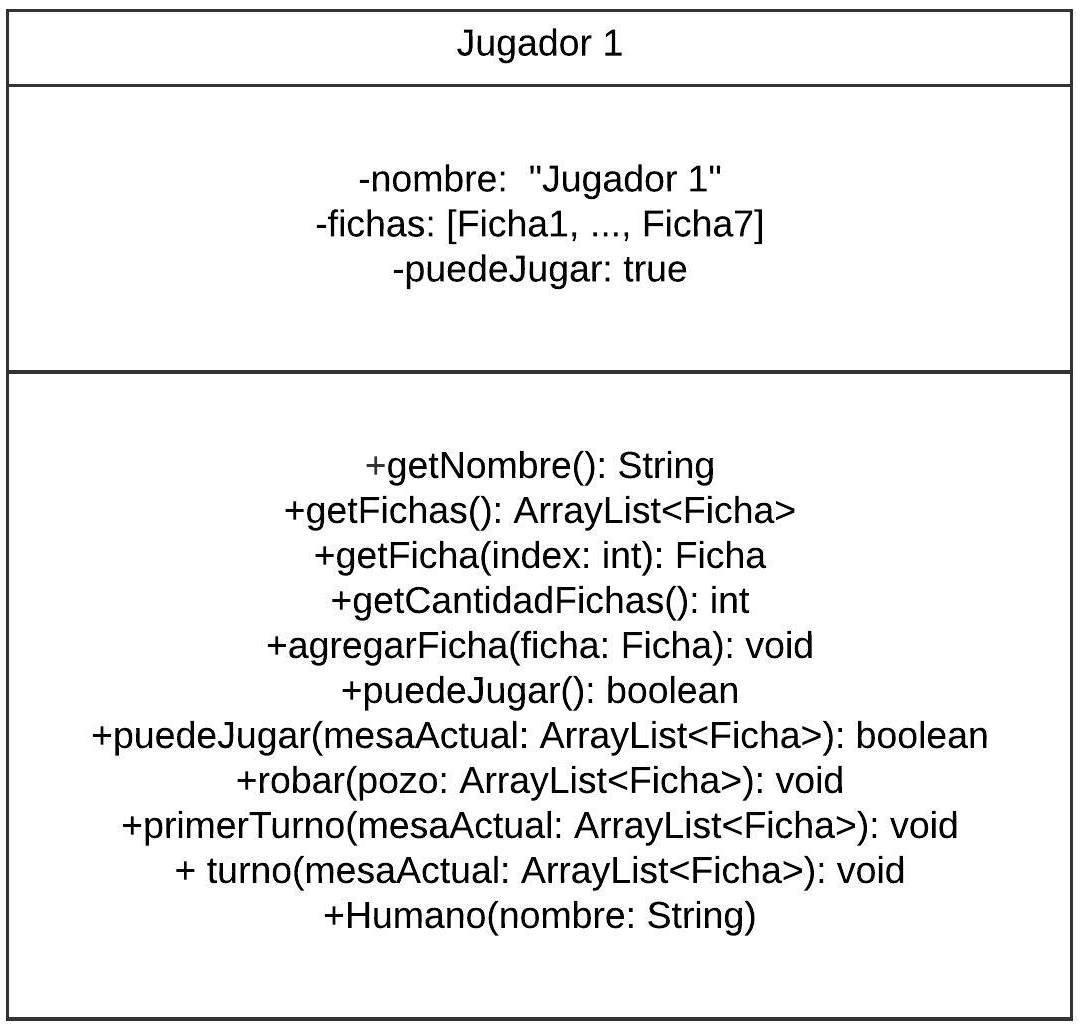
\includegraphics[height=6cm]{umlo3.png}
      \caption{UML de objeto \textit{Jugador1}}
    \end{minipage}
    \begin{minipage}[r]{0.45\textwidth} 
      \centering
      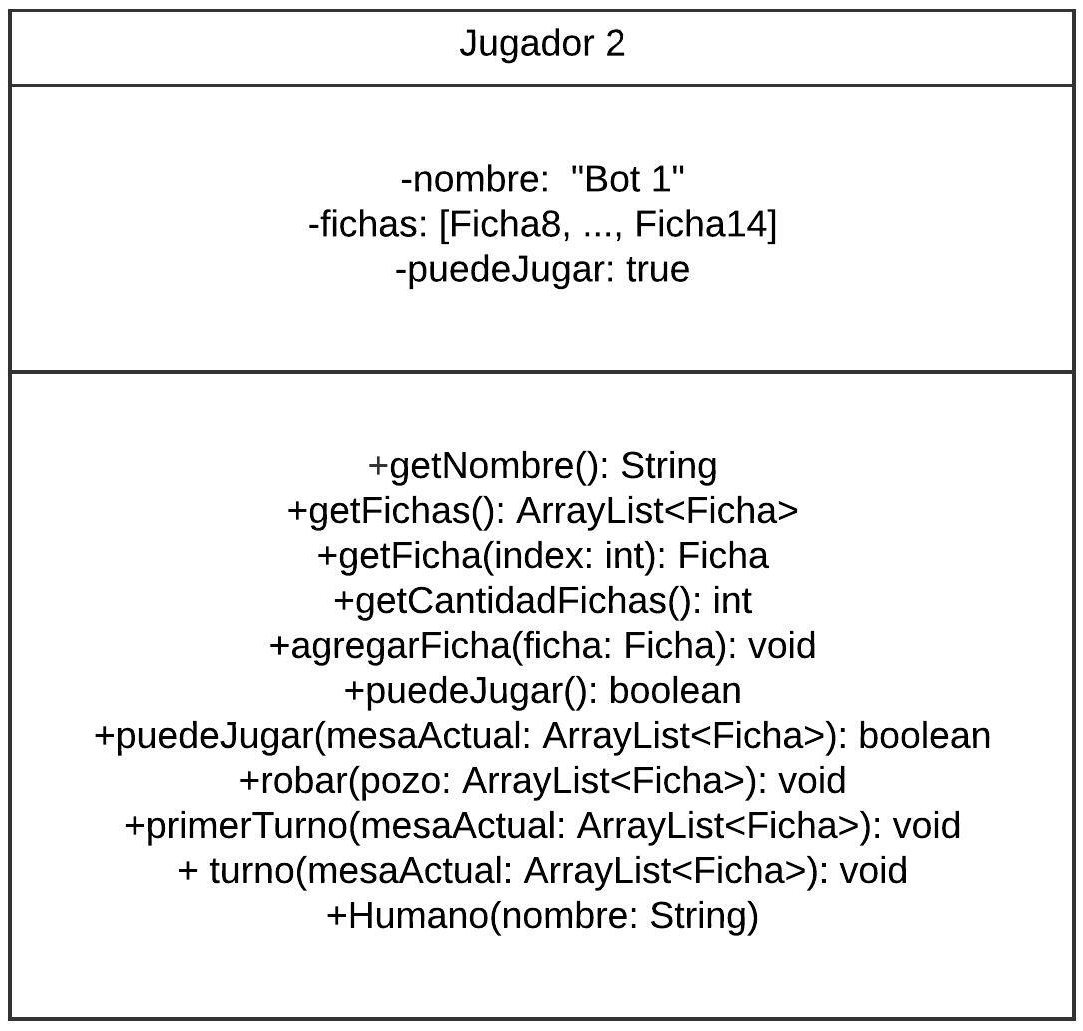
\includegraphics[height=6cm]{umlo4.png}
      \caption{UML de objeto \textit{Jugador1}}
    \end{minipage}
  \end{figure}

  \begin{figure}[h!]
    \centering
    \begin{minipage}[l]{0.45\textwidth}
      \centering
      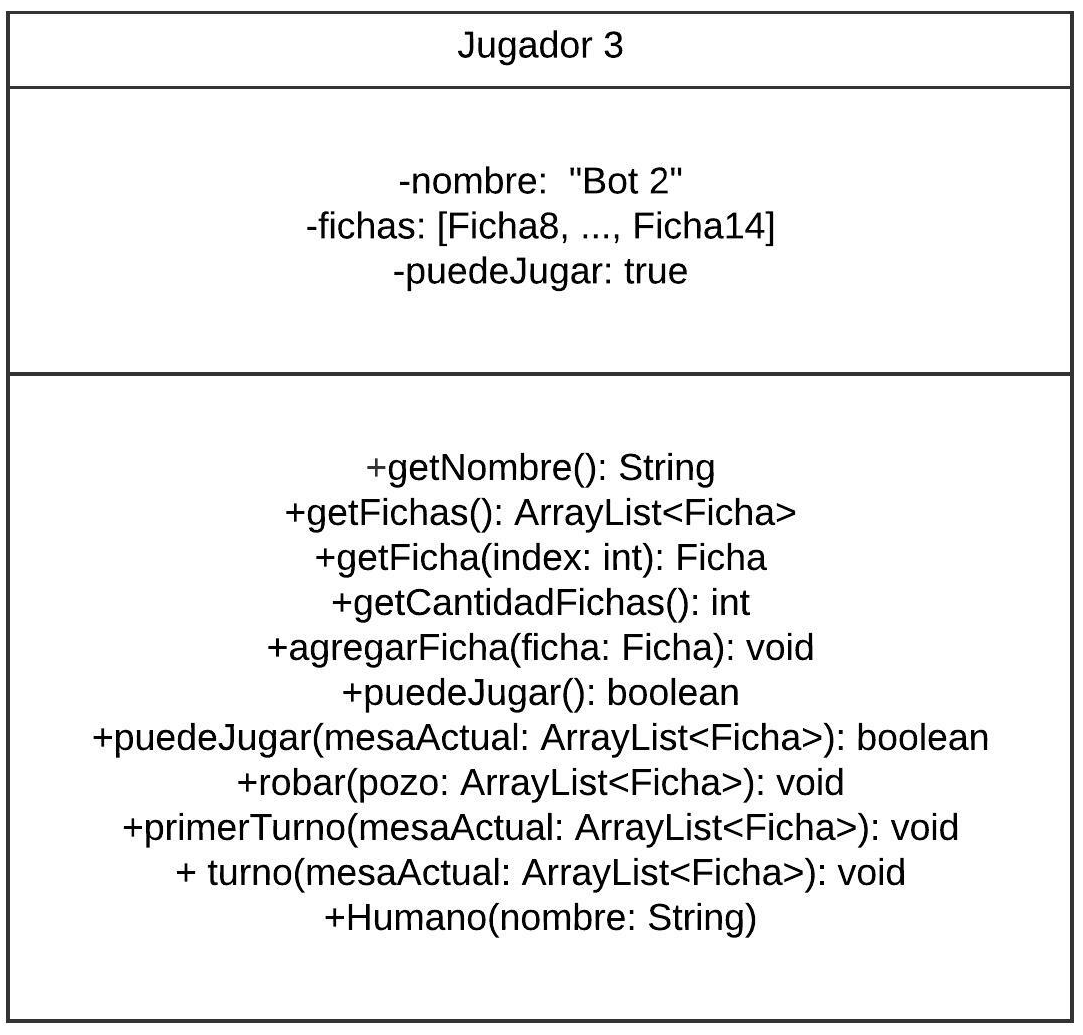
\includegraphics[height=6cm]{umlo5.png}
      \caption{UML de objeto \textit{Jugador1}}
    \end{minipage}
    \begin{minipage}[r]{0.45\textwidth}
      \centering
      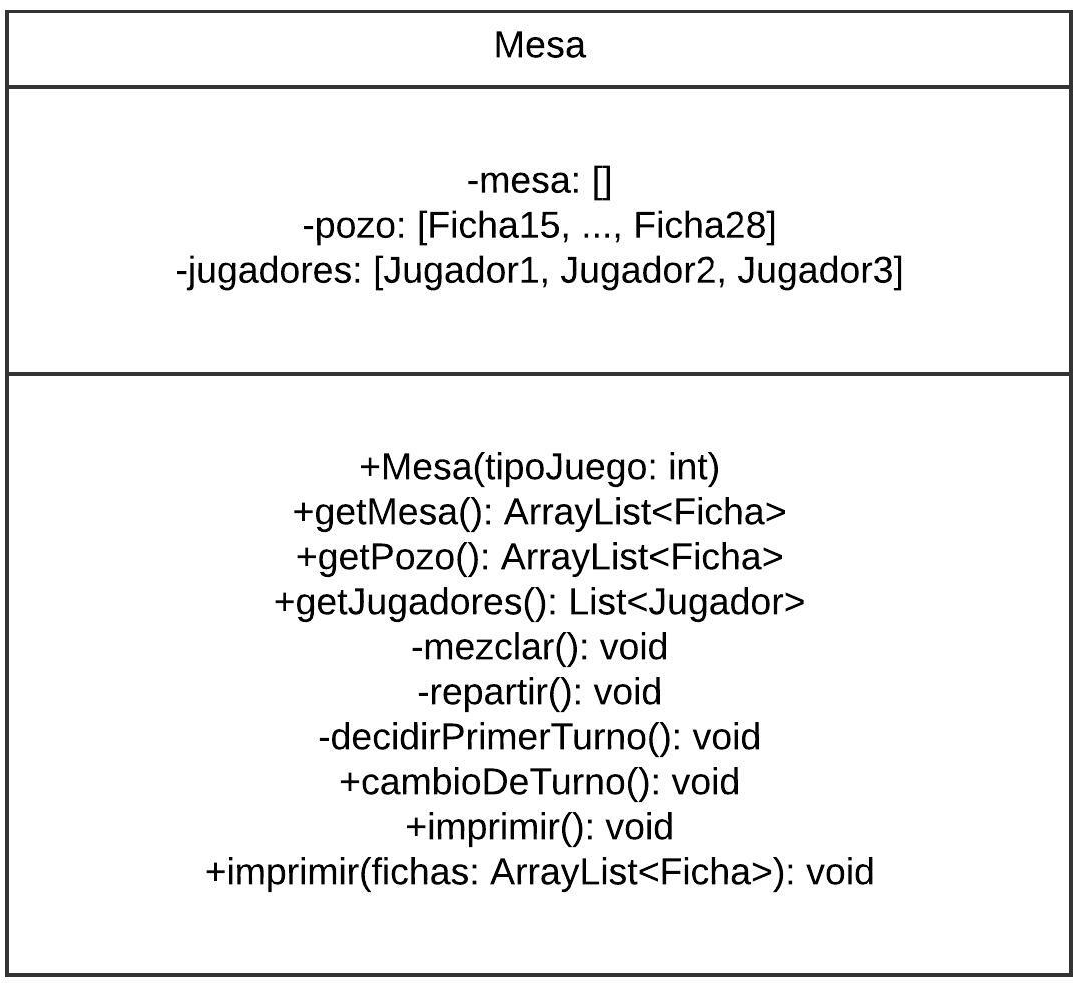
\includegraphics[height=6cm]{umlo6.png}
      \caption{UML de objeto \textit{Mesa}} 
    \end{minipage}
  \end{figure}

  \subsection{Diagrama UML de casos de uso}
  \begin{figure}[h!]
    \centering
    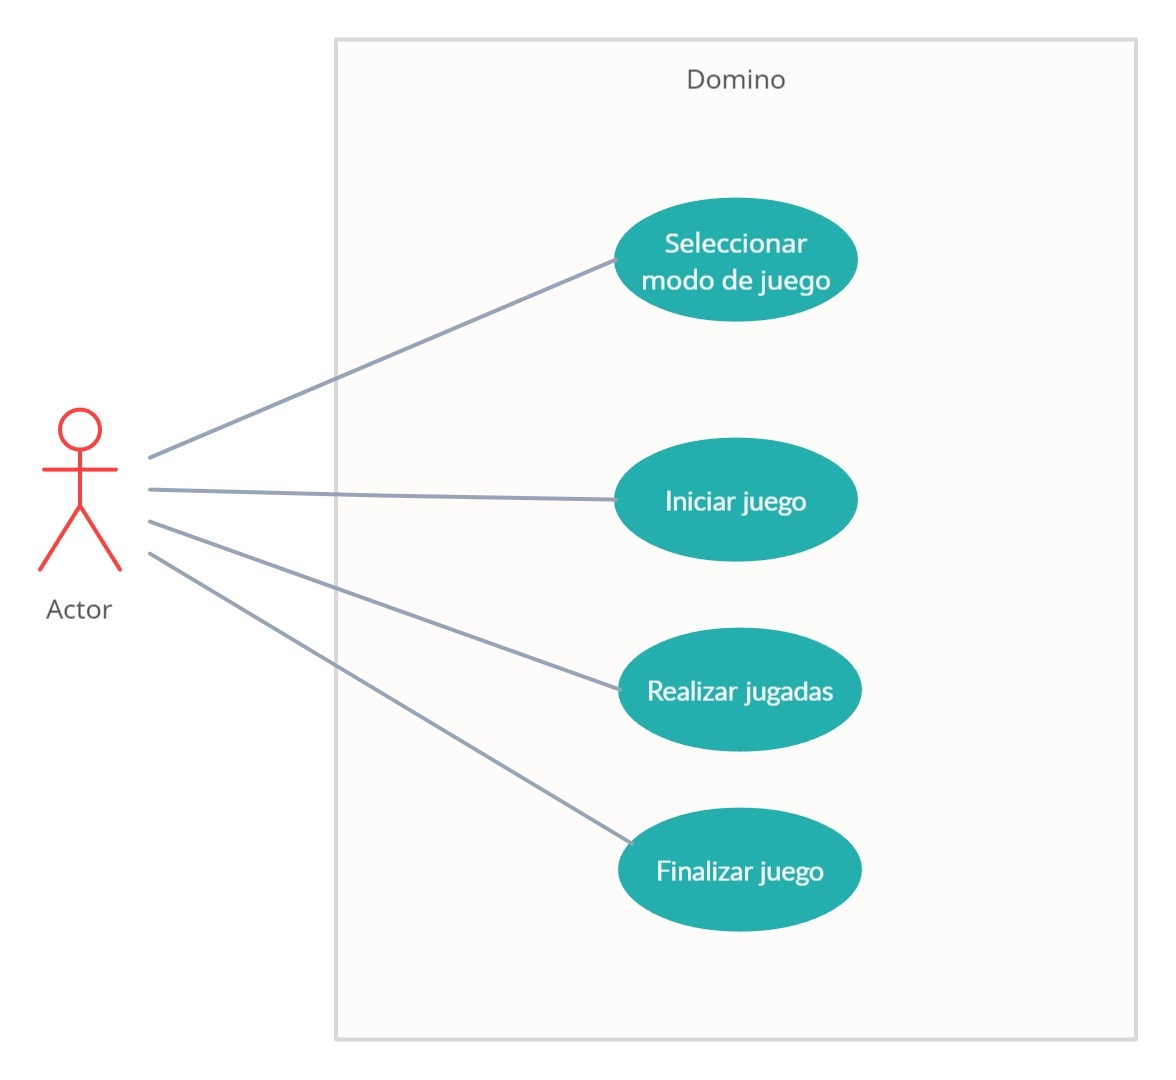
\includegraphics[width=0.75\textwidth]{umlcu.jpg}
    \caption{UML de casos de uso}
  \end{figure}

  \newpage
  \subsection{Diagrama UML de estados de hilos}
  \begin{figure}[h!]
    \centering
    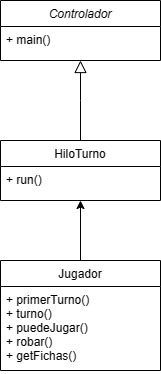
\includegraphics[width=0.25\textwidth]{umlh.jpg}
    \caption{UML de estados de hilos}
  \end{figure}


  \subsection{Diagrama UML de MVC}  
  \begin{sidewaysfigure}
    \centering
    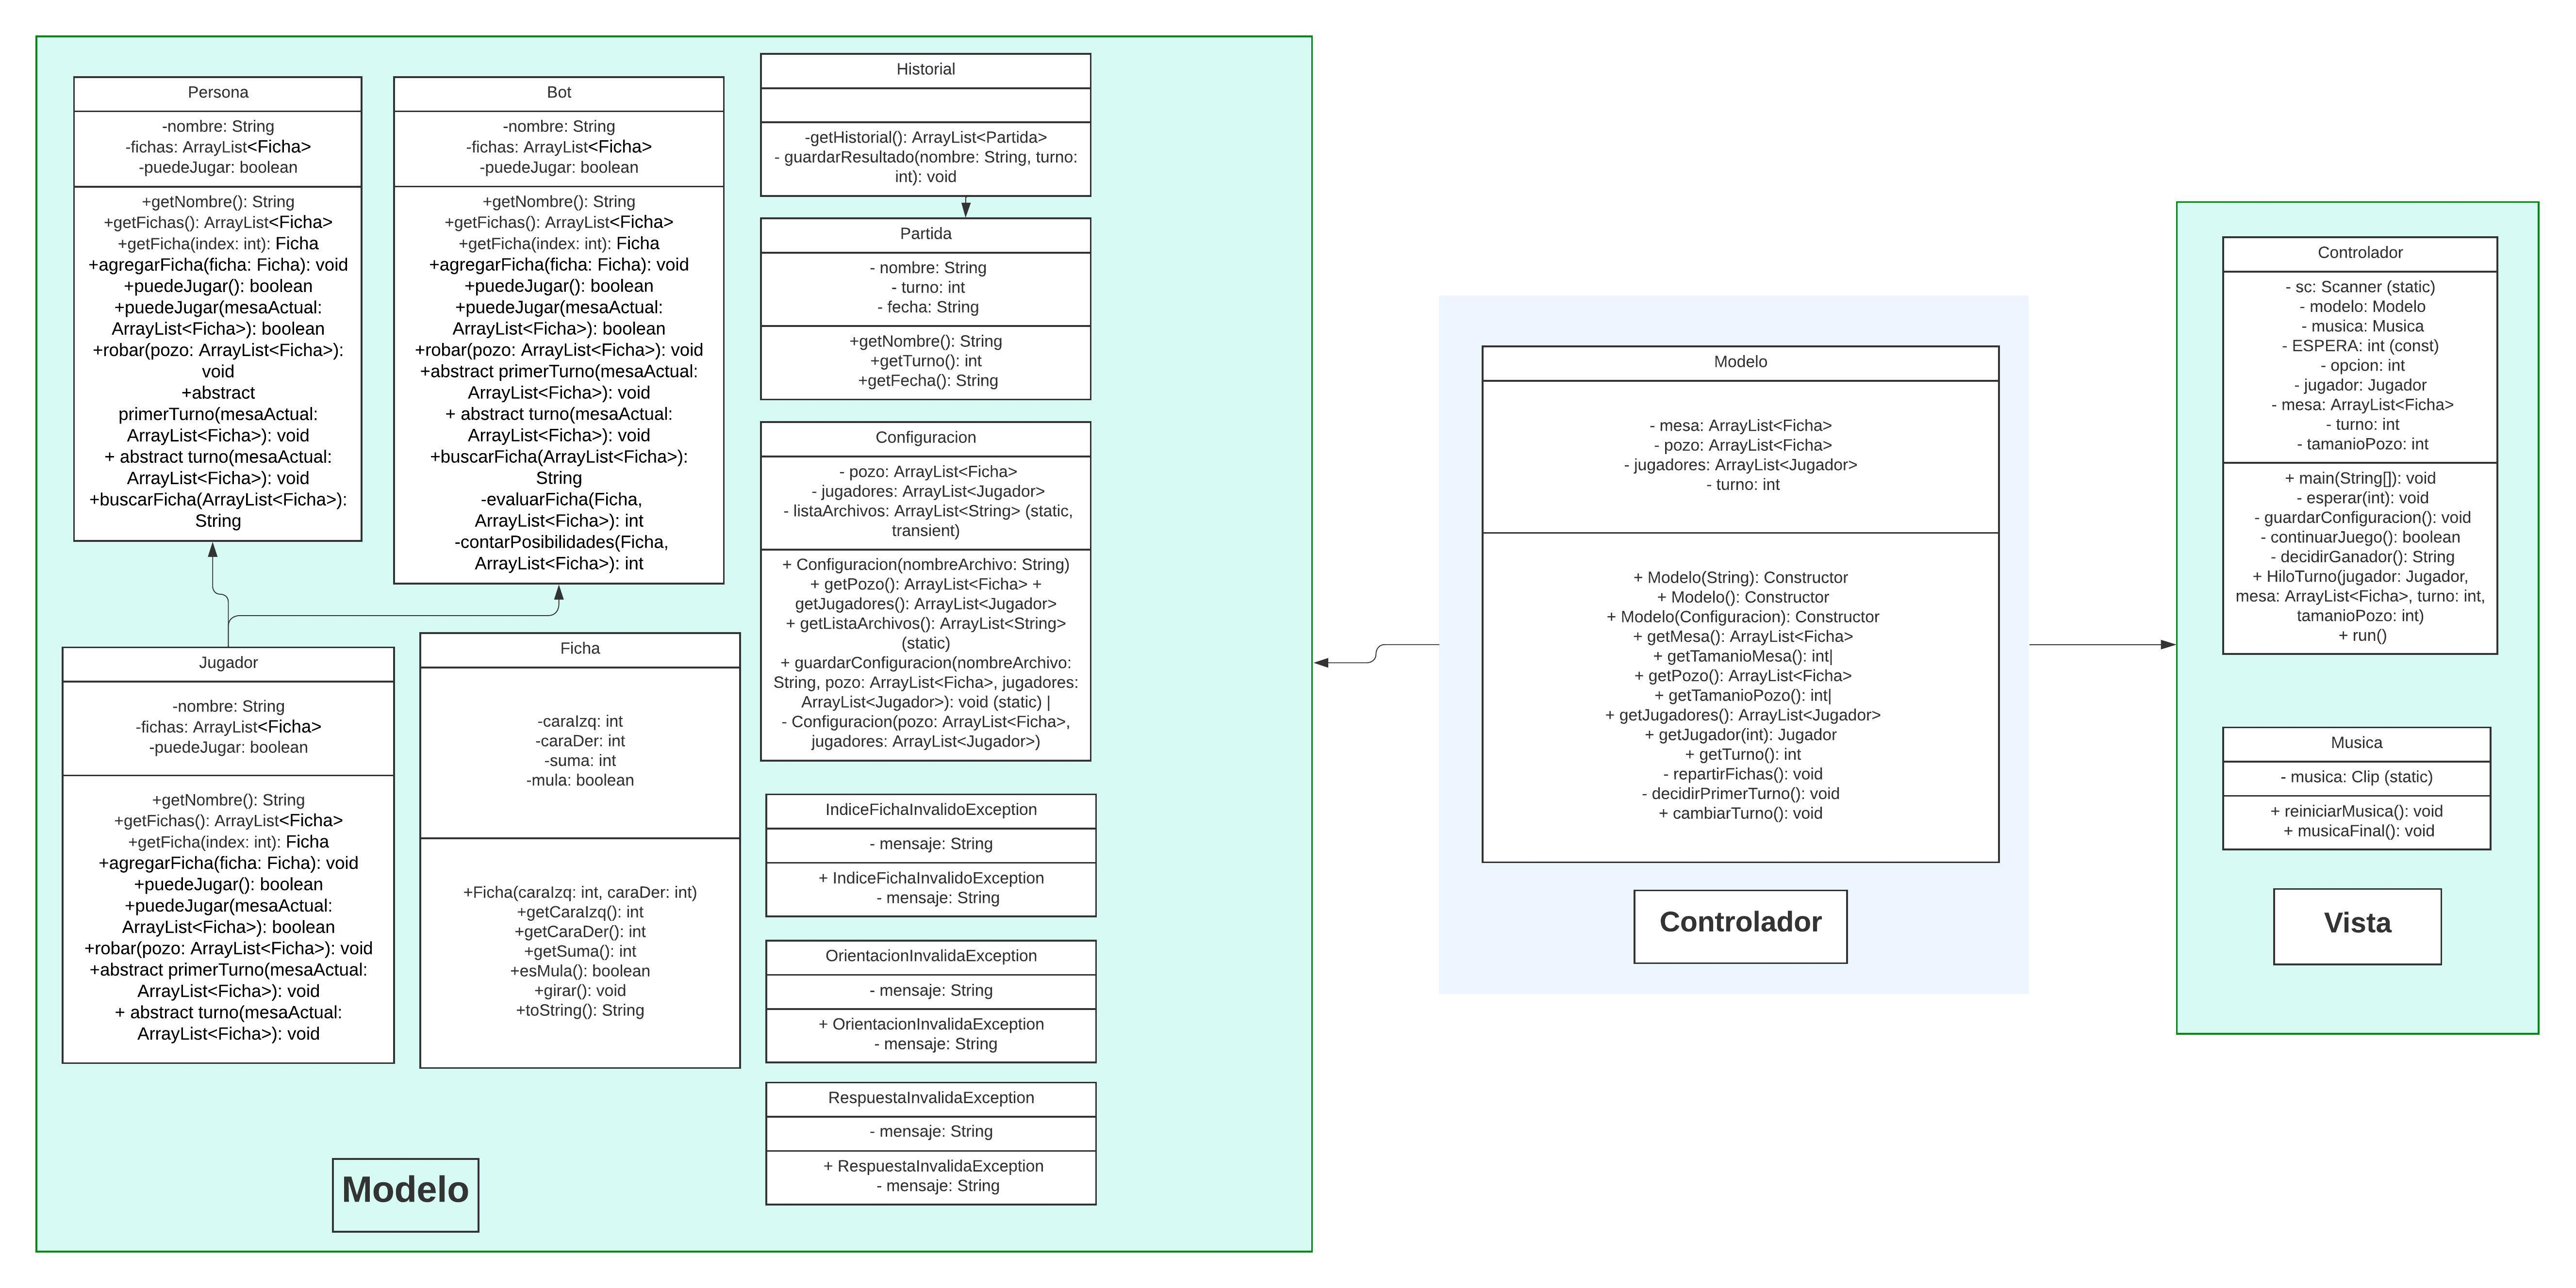
\includegraphics[width=\textheight]{umlmvc.jpeg} 
    \caption{UML de MVC}
  \end{sidewaysfigure}
  \newpage

  \subsection{Diagrama UML de actividades}
  \begin{figure}[h!]
    \centering
    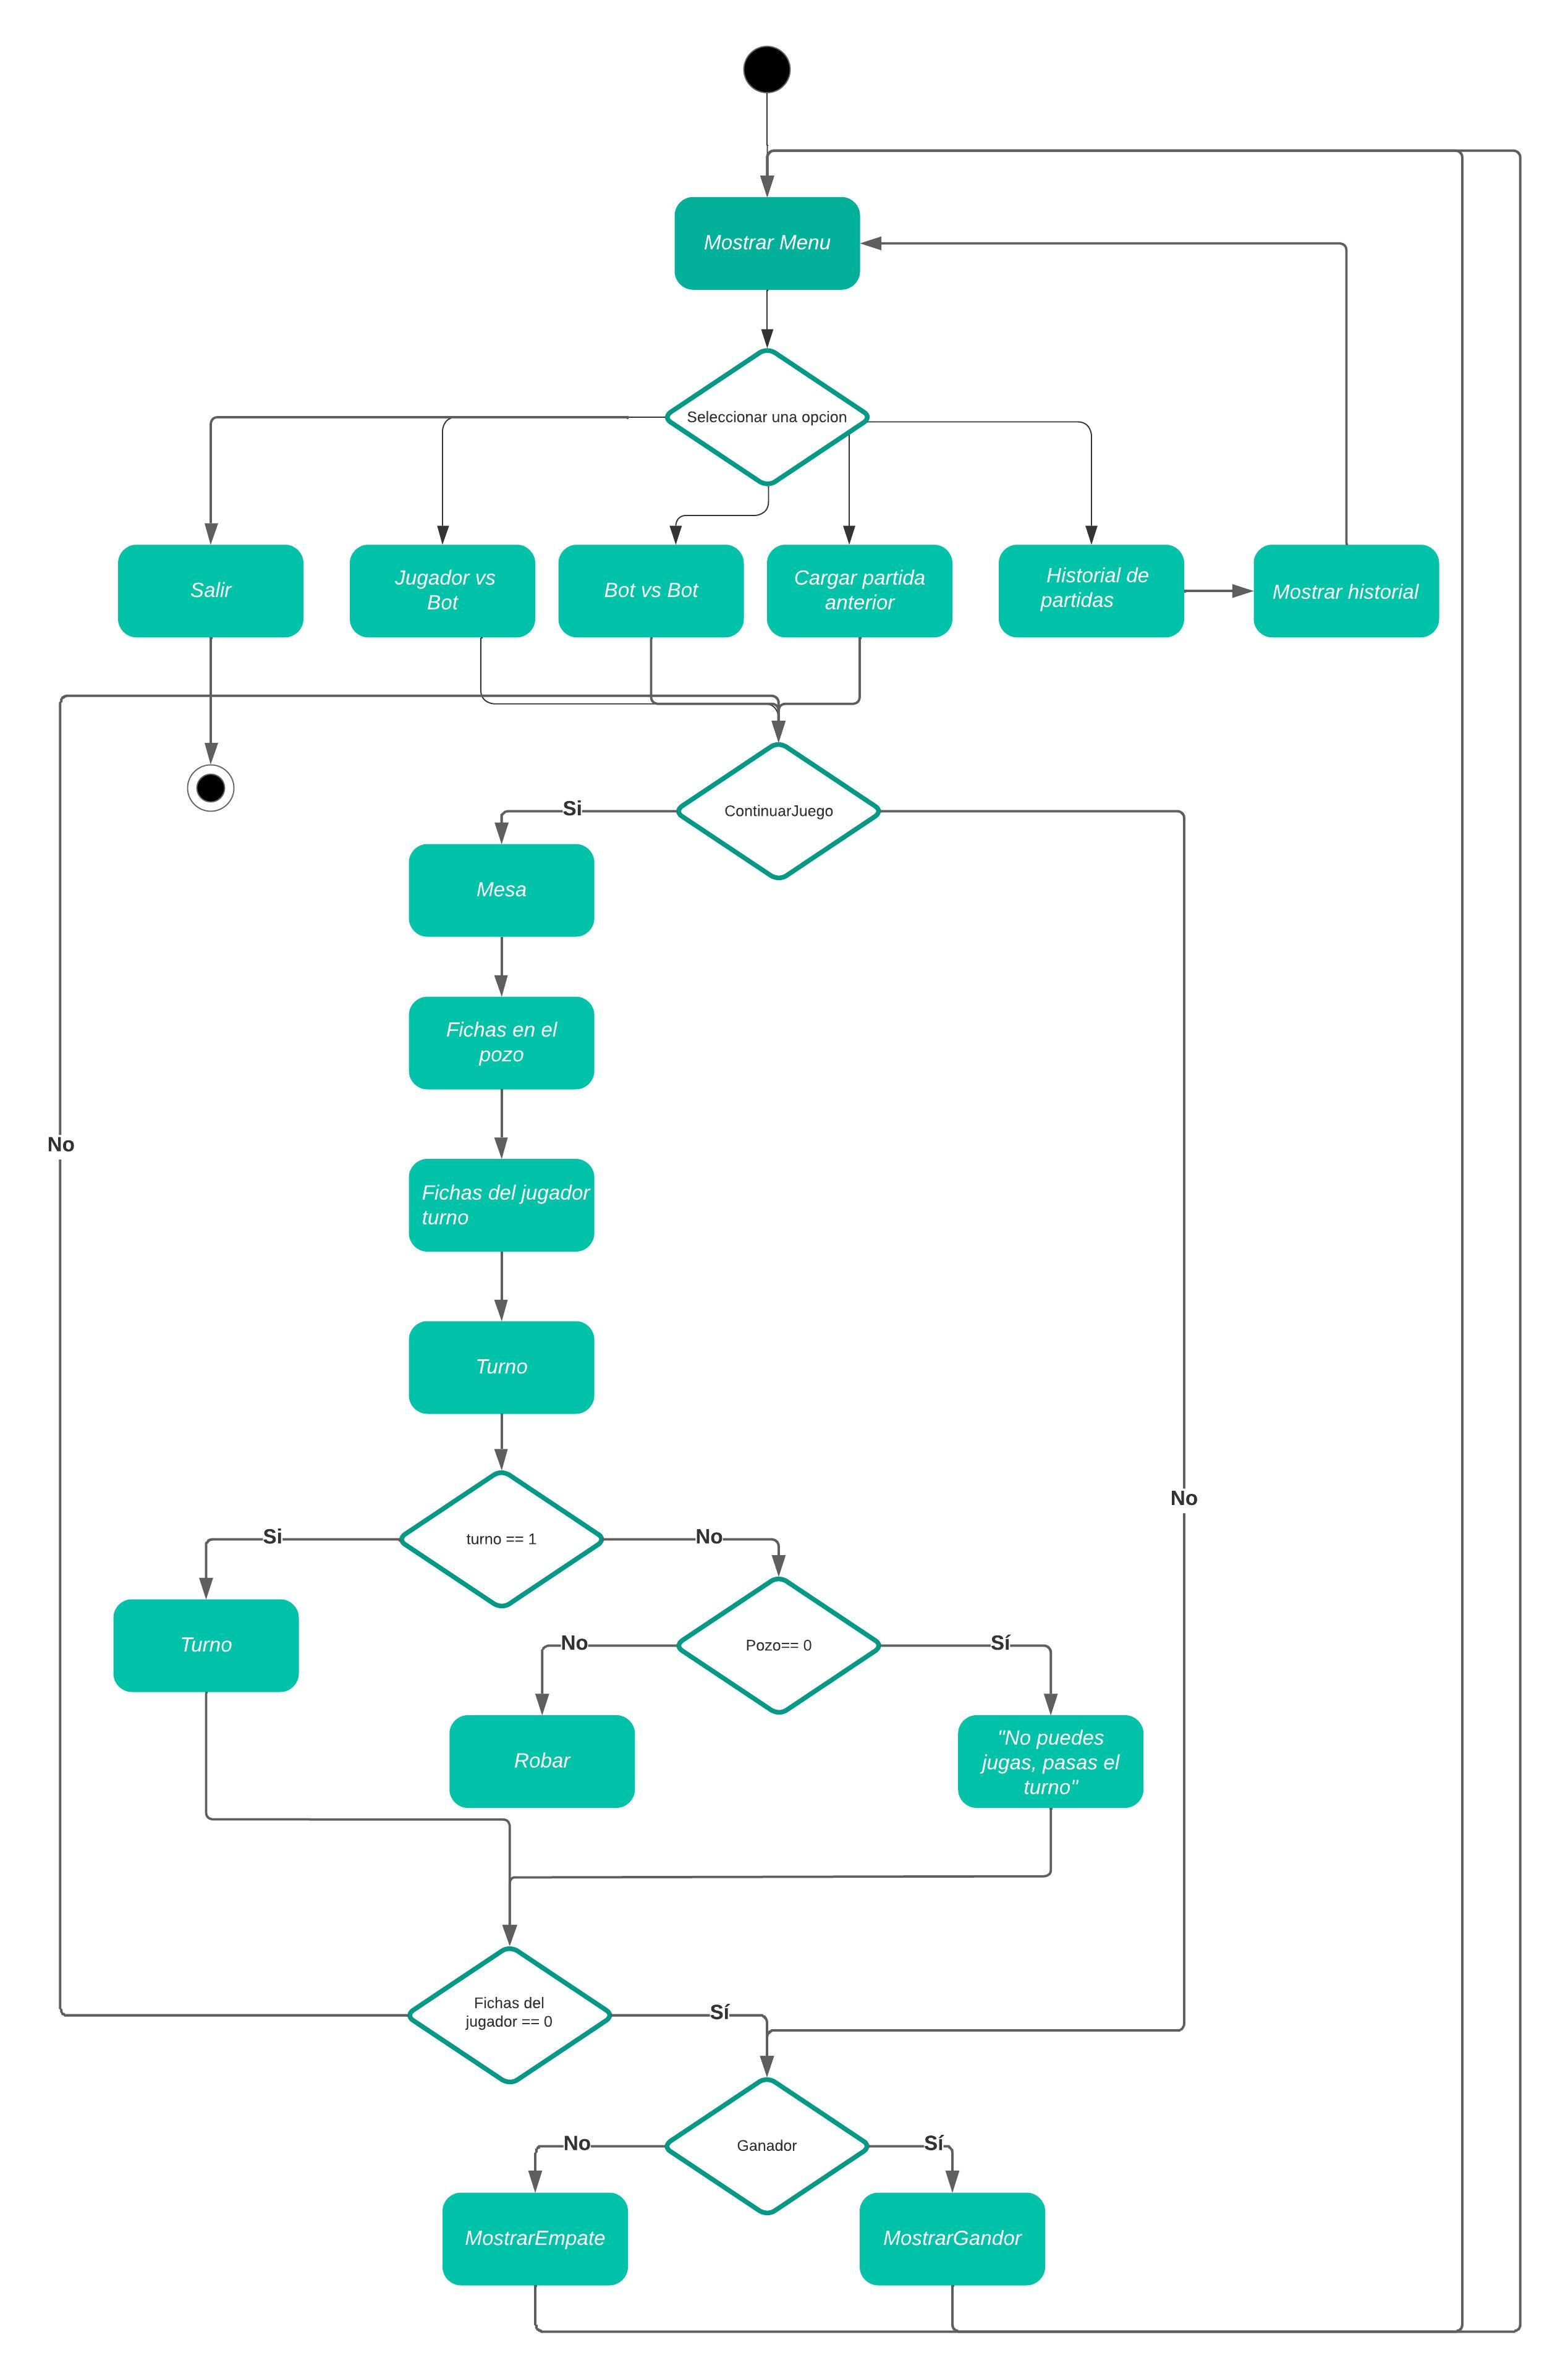
\includegraphics[width=0.75\textwidth]{umlact.jpeg}
    \caption{UML de actividades}
  \end{figure}

  \newpage
  \subsection{Diagrama UML de componentes}
  \begin{figure}[h!]
    \centering
    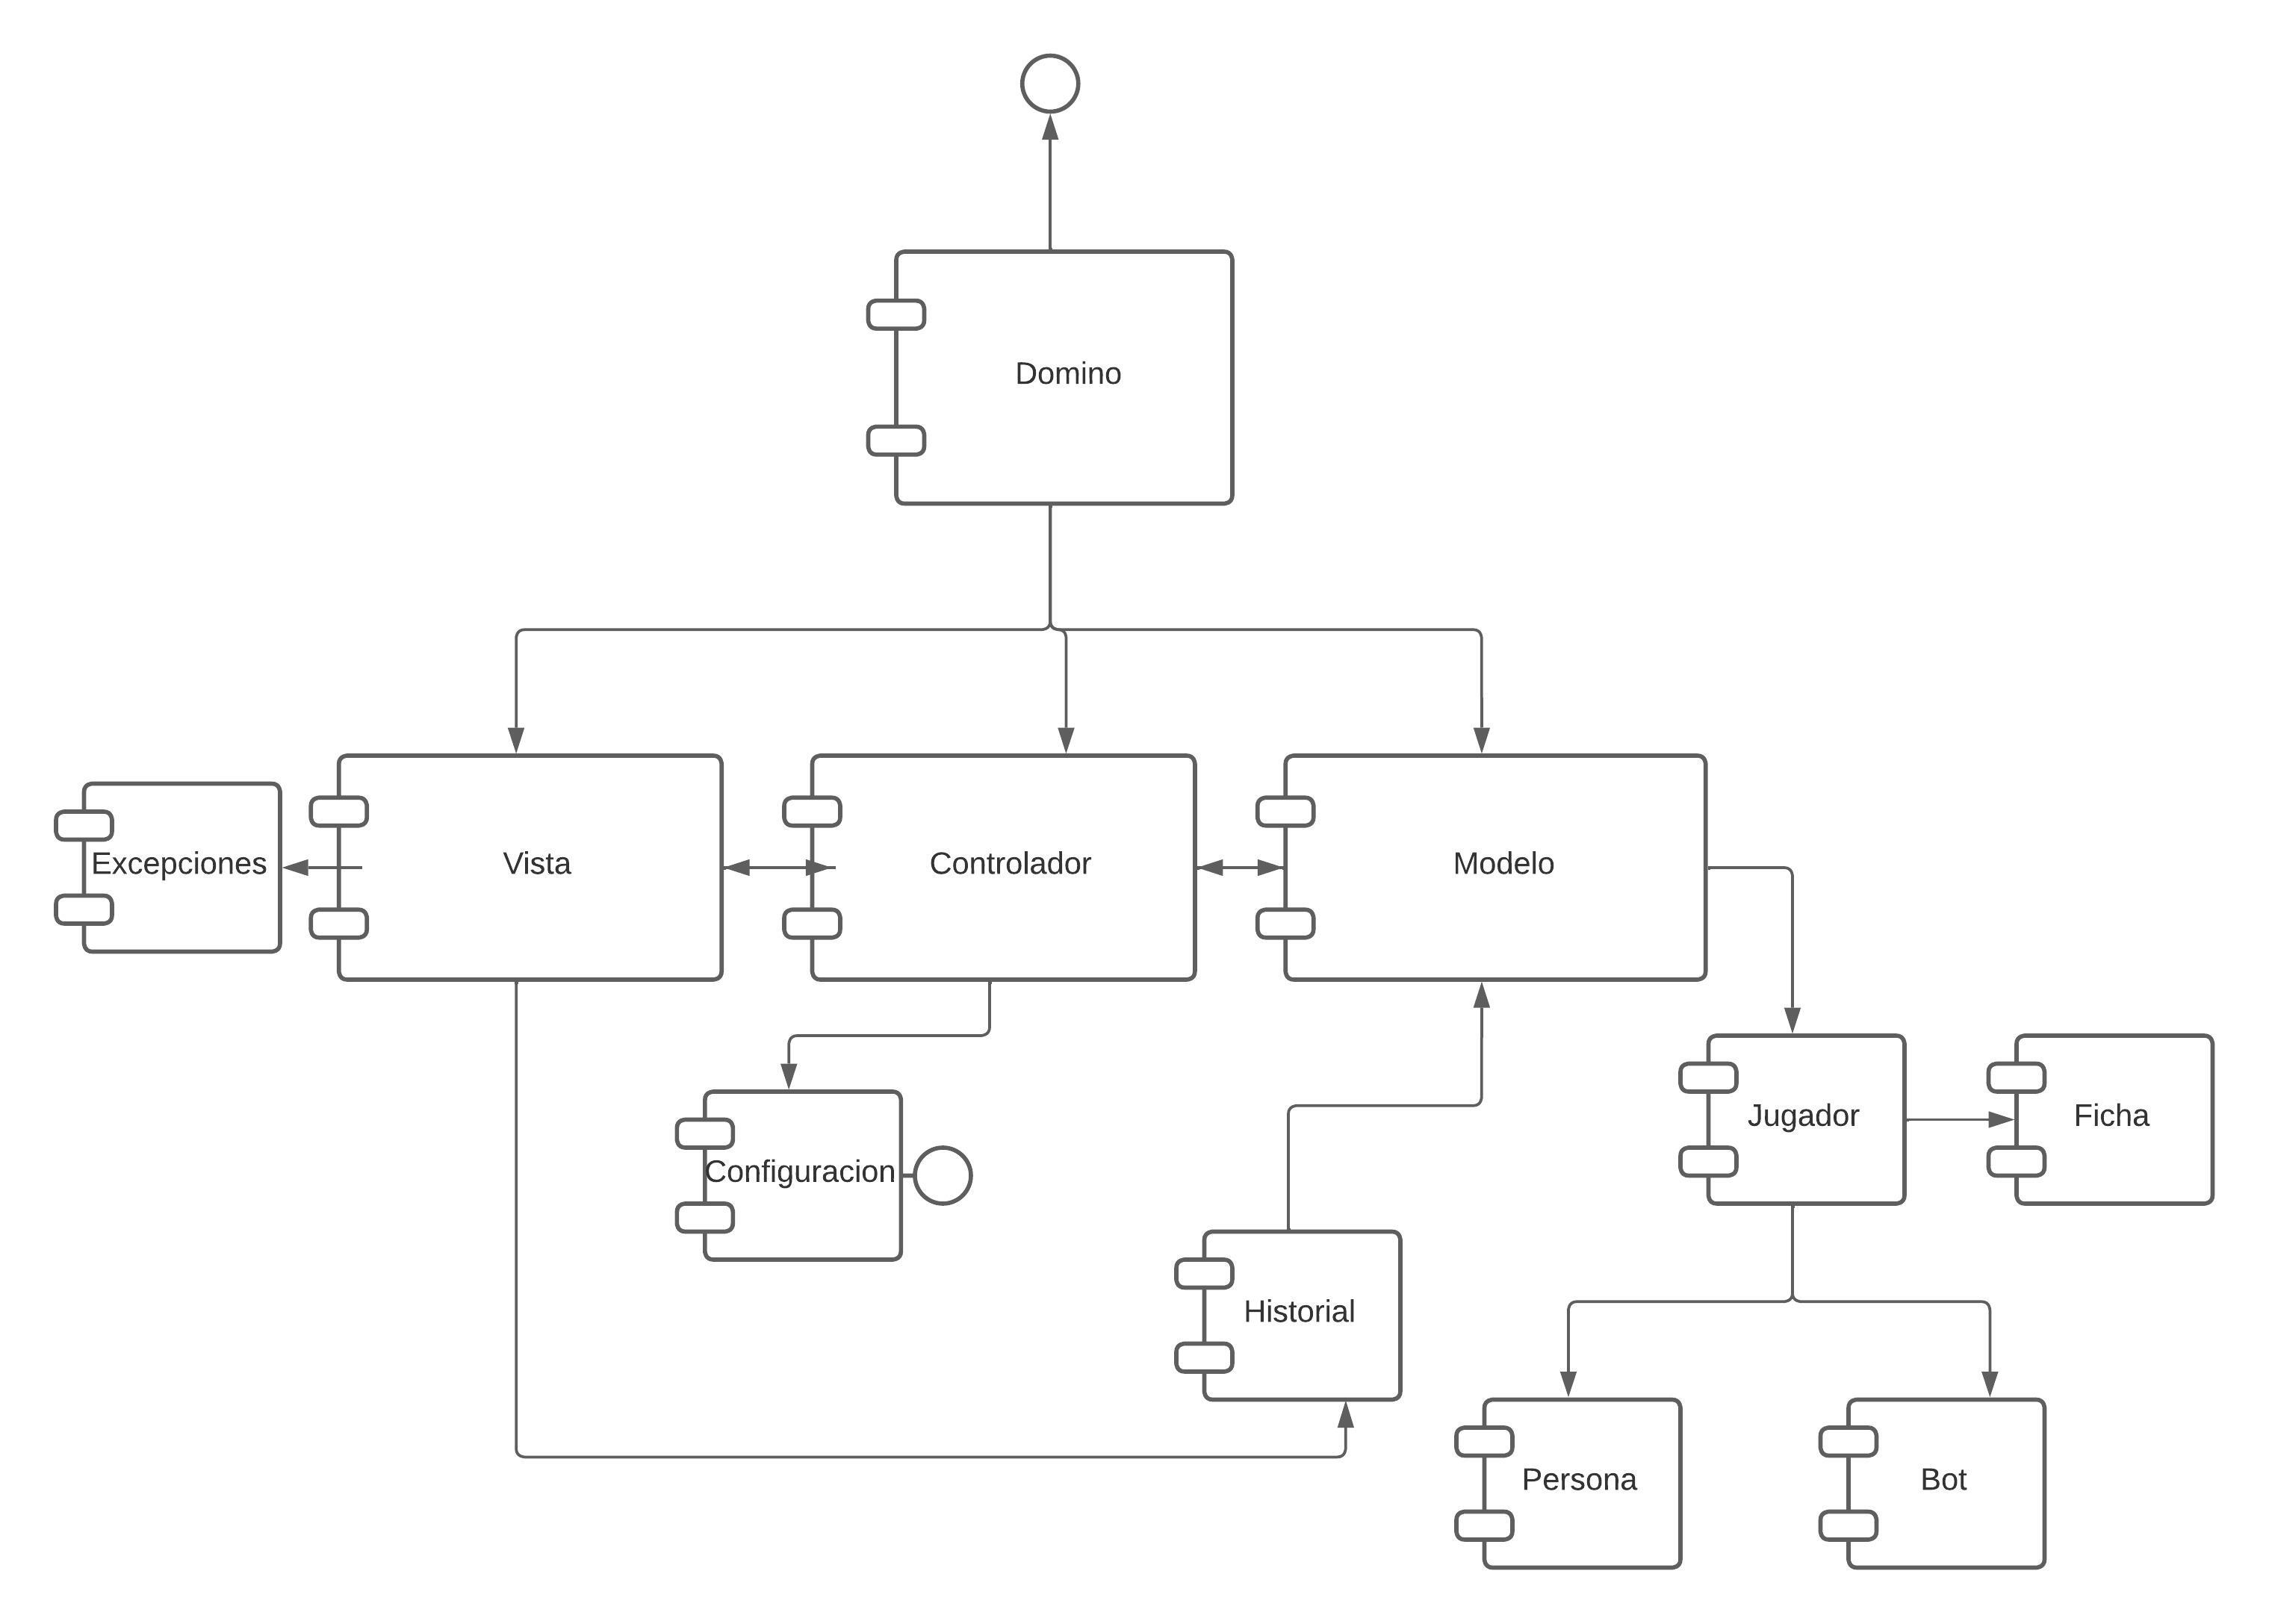
\includegraphics[width=\textwidth]{umlcomp.jpeg}
    \caption{UML de componentes}
  \end{figure}

  \subsection{Código fuente}
  \subsubsection{Ficha.java}
  \begin{lstlisting}
package domino;

import java.io.Serializable;

/**
 * Representa una ficha de domino con dos caras.
 * Cada cara tiene un numero, y la ficha puede ser una "mula" si ambas caras son iguales.
 */
public class Ficha implements Serializable {
  private int caraIzq;
  private int caraDer;
  private int suma;
  private boolean mula;

  /**
    * Constructor que recibe las dos caras de la ficha.
    * @param caraIzq Numero de la cara izquierda.
    * @param caraDer Numero de la cara derecha.
    */
  public Ficha(int caraIzq, int caraDer) {
    this.caraIzq = caraIzq;
    this.caraDer = caraDer;
    this.suma = caraIzq + caraDer;
    this.mula = (caraIzq == caraDer);
  }

  /**
    * Obtiene el numero de la cara izquierda.
    * @return Numero de la cara izquierda.
    */
  public int getCaraIzq() {
    return caraIzq;
  }

  /**
    * Obtiene el numero de la cara derecha.
    * @return Numero de la cara derecha.
    */
  public int getCaraDer() {
    return caraDer;
  }

  /**
    * Obtiene la suma de las caras.
    * @return Suma de las caras.
    */
  public int getSuma() {
    return suma;
  }

  /**
    * Comprueba si la ficha es una mula (ambas caras son iguales).
    * @return `true` si la ficha es una mula, `false` si no.
    */
  public boolean esMula() {
    return mula;
  }

  /**
    * Gira la ficha intercambiando las caras izquierda y derecha.
    */
  public void girar() {
    int aux = caraIzq;
    caraIzq = caraDer;
    caraDer = aux;
  }

  /**
    * Representacion en cadena de la ficha con el formato [caraIzq|caraDer].
    * @return Cadena que representa la ficha.
    */
  @Override
  public String toString() {
    return "[" + caraIzq + "|" + caraDer + "]";
  }
}
  \end{lstlisting}

  \subsubsection{Jugador.java}
  \begin{lstlisting}
package domino;

import java.util.ArrayList;
import java.io.Serializable;

/**
 * Clase abstracta que representa un jugador de domino.
 */
public abstract class Jugador implements Serializable {
  protected String nombre;
  protected ArrayList<Ficha> fichas = new ArrayList<>();
  protected boolean puedeJugar = true;

  /**
    * Obtiene el nombre del jugador.
    * @return Nombre del jugador.
    */
  public String getNombre() {
    return nombre;
  }

  /**
    * Obtiene las fichas del jugador.
    * @return Lista de fichas del jugador.
    */
  public ArrayList<Ficha> getFichas() {
    return fichas;
  }

  /**
    * Obtiene una ficha especifica del jugador.
    * @param i Indice de la ficha.
    * @return Ficha del jugador.
    */
  public Ficha getFicha(int i) {
    return fichas.get(i);
  }

  /**
    * Agrega una ficha a las fichas del jugador.
    * @param ficha Ficha a agregar.
    */
  public void agregarFicha(Ficha ficha) {
    fichas.add(ficha);
  }

  /**
    * Indica si el jugador puede jugar.
    * @return `true` si el jugador puede jugar, `false` si no.
    */
  public boolean puedeJugar() {
    return puedeJugar;
  }

  /**
    * Verifica si el jugador puede jugar con las fichas disponibles.
    * @param mesa Fichas de la mesa actual.
    * @return `true` si el jugador puede jugar, `false` si no.
    */
  public boolean puedeJugar(ArrayList<Ficha> mesa) {
    puedeJugar = fichas.stream().anyMatch(ficha ->
      ficha.getCaraIzq() == mesa.get(0).getCaraIzq() ||
      ficha.getCaraDer() == mesa.get(0).getCaraIzq() ||
      ficha.getCaraIzq() == mesa.get(mesa.size() - 1).getCaraDer() ||
      ficha.getCaraDer() == mesa.get(mesa.size() - 1).getCaraDer()
    );
    return puedeJugar;
  }

  /**
    * Roba una ficha del pozo y la agrega a las fichas del jugador.
    * @param pozo Pozo de fichas.
    */
  public void robar(ArrayList<Ficha> pozo) {
    fichas.add(pozo.get(0));
    pozo.remove(0);
  }

  /**
    * Realiza la jugada del primer turno, eligiendo la ficha mas alta.
    * @param mesa Fichas de la mesa.
    */
  public void primerTurno(ArrayList<Ficha> mesa) {
    int indice = -1;
    int max = -1;

    for (Ficha ficha : fichas) {
      if (ficha.esMula() && ficha.getSuma() > max) {
        max = ficha.getSuma();
        indice = fichas.indexOf(ficha);
      }
    }

    if (indice != -1)
      System.out.println("\n" + nombre + " juega la mula mas alta: " + fichas.get(indice));
    else {
      for (Ficha ficha : fichas) {
        if (ficha.getSuma() > max) {
          max = ficha.getSuma();
          indice = fichas.indexOf(ficha);
        }
      }
      System.out.println("\n" + nombre + " juega la ficha mas alta: " + fichas.get(indice));
    }

    mesa.add(fichas.get(indice));
    fichas.remove(indice);
  }

  /**
    * Realiza la jugada en un turno normal.
    * @param mesa Fichas de la mesa.
    */
  public final void turno(ArrayList<Ficha> mesa) {
    int indice = -1;
    char orientacion;
    String respuesta;
    boolean validacion;

    do {
      respuesta = buscarFicha(mesa);
      orientacion = respuesta.charAt(0);
      indice = Integer.parseInt(respuesta.substring(1));
      validacion = validarFicha(mesa, indice, orientacion);
      if (!validacion)
        System.out.println("Ficha invalida\n");
    } while (!validacion);

    System.out.println("\n" + nombre + " juegas la ficha: " + (indice + 1) + " - " + fichas.get(indice));

    jugarFicha(mesa, indice, orientacion);
  }

  /**
    * Metodo abstracto para buscar la ficha a jugar.
    * @param mesa Fichas de la mesa.
    * @return Representacion de la jugada (orientacion + indice).
    */
  protected abstract String buscarFicha(ArrayList<Ficha> mesa);

  /**
    * Valida si una ficha puede ser jugada en la mesa en la orientacion indicada.
    * @param mesa Fichas de la mesa actual.
    * @param indice indice de la ficha a jugar.
    * @param orientacion Orientacion de la ficha ('i' o 'd').
    * @return true si la ficha es valida para jugar, false si no.
    */
  private boolean validarFicha(ArrayList<Ficha> mesa, int indice, char orientacion) {
    switch (orientacion) {
      case 'i':
        if (fichas.get(indice).getCaraIzq() == mesa.get(0).getCaraIzq()) {
          fichas.get(indice).girar();
          return true;
        }
        if (fichas.get(indice).getCaraDer() == mesa.get(0).getCaraIzq()) 
          return true;
        return false;

      case 'd':
        if (fichas.get(indice).getCaraDer() == mesa.get(mesa.size() - 1).getCaraDer()) {
          fichas.get(indice).girar();
          return true;
        }
        if (fichas.get(indice).getCaraIzq() == mesa.get(mesa.size() - 1).getCaraDer()) 
          return true;
        return false;

      default:
        return false;   
    }
  }

  /**
    * Juega la ficha en la mesa segun la orientacion.
    * Este metodo es sincronizado para evitar que dos jugadores jueguen la misma ficha.
    * @param mesa Fichas de la mesa.
    * @param indice Indice de la ficha a jugar.
    * @param orientacion Orientacion de la ficha ('i' o 'd').
    */
  private synchronized void jugarFicha(ArrayList<Ficha> mesa, int indice, char orientacion) {
    if (orientacion == 'i')
      mesa.add(0, fichas.get(indice));
    else if (orientacion == 'd')
      mesa.add(fichas.get(indice));
    fichas.remove(indice);
  }
}
  \end{lstlisting} 

  \subsubsection{Persona.java}
  \begin{lstlisting}
package domino;

import java.util.ArrayList;
import java.util.Scanner;

/**
 * Esta clase representa un jugador humano de domino.
 */
public class Persona extends Jugador {
  /**
    * Constructor de la clase Persona.
    * @param nombre Nombre del jugador.
    */
  public Persona(String nombre) {
    this.nombre = nombre;
  }

  /**
    * Metodo sobreescrito para permitir al jugador humano seleccionar una ficha
    * para jugar y la orientacion en la que desea colocarla.
    * @param mesaActual Lista de fichas en la mesa actual.
    * @return Cadena que representa la accion del jugador (orientacion + indice).
    */
  @Override
  protected String buscarFicha(ArrayList<Ficha> mesaActual) {
    Scanner sc = new Scanner(System.in);
    int indice = -1;
    char orientacion = ' ';

    do {
      try {
        System.out.println("\nQue ficha deseas jugar? (1 - " + fichas.size() + ")");
        System.out.print("$ ");
        indice = sc.nextInt() - 1;
        if (indice < 0 || indice >= fichas.size())
          throw new IndiceFichaInvalidoException("Indice de ficha no valido. Debe ser entre 1 y " + fichas.size());
      } catch (IndiceFichaInvalidoException e) {
          System.out.println(e.getMessage() + "\n");
      }
    } while (indice < 0 || indice >= fichas.size());
    
    do {
      try {
        System.out.println("Donde la quieres jugar? (i o d)");
        System.out.print("$ ");
        orientacion = sc.next().charAt(0);
        if (orientacion != 'i' && orientacion != 'd') 
          throw new OrientacionInvalidaException("Orientacion no valida. Debe ser 'i' o 'd'.");
      } catch (OrientacionInvalidaException e) {
        System.out.println(e.getMessage() + "\n");
      }
    } while (orientacion != 'i' && orientacion != 'd');

    return orientacion + "" + indice;
  }
}
  \end{lstlisting}

  \subsubsection{Bot.java}
  \begin{lstlisting}
package domino;

import java.util.ArrayList;

/**
 * Esta clase representa un jugador bot de domino.
 * Extiende la clase abstracta Jugador.
 */
public class Bot extends Jugador {
  /**
    * Constructor de la clase Bot.
    * @param nombre Nombre del bot.
    */
  public Bot(String nombre) {
    this.nombre = nombre;
  }

  /**
    * Metodo para que el bot elija una ficha para jugar en la mesa.
    * Evalua sus fichas disponibles y selecciona la que maximiza sus posibilidades de juego.
    * @param mesa La lista de fichas en la mesa.
    * @return Intruccion que representa la eleccion de la ficha y su orientacion ('i' o 'd').
    */
  @Override
  protected String buscarFicha(ArrayList<Ficha> mesa) {
    Ficha mejorFicha = null;
    int mejorPuntuacion = Integer.MIN_VALUE;

    for (Ficha ficha : fichas) {
      int puntuacion = evaluarFicha(ficha, mesa);
      if (puntuacion > mejorPuntuacion) {
        mejorPuntuacion = puntuacion;
        mejorFicha = ficha;
      }
    }

    if (mejorFicha != null) {
      int indice = fichas.indexOf(mejorFicha);
      if (mejorFicha.getCaraIzq() == mesa.get(0).getCaraIzq()) 
          return "i" + indice;
      else if (mejorFicha.getCaraDer() == mesa.get(0).getCaraIzq()) 
          return "i" + indice;
      else if (mejorFicha.getCaraIzq() == mesa.get(mesa.size() - 1).getCaraDer()) 
          return "d" + indice;
      else if (mejorFicha.getCaraDer() == mesa.get(mesa.size() - 1).getCaraDer()) 
          return "d" + indice;
    }

    return elegirFichaGenerica(mesa);
  }

  /**
    * Evalua una ficha especifica en funcion de las posibilidades de juego en la mesa.
    * @param ficha Ficha a evaluar.
    * @param mesa Lista de fichas en la mesa.
    * @return Cantidad de posibilidades de juego para la ficha.
    */
  private int evaluarFicha(Ficha ficha, ArrayList<Ficha> mesa) {
    int cantidadPosibilidades = contarPosibilidades(ficha, mesa);
    return cantidadPosibilidades;
  }

  /**
    * Cuenta la cantidad de posibilidades de juego para una ficha en la mesa.
    * @param ficha Ficha a evaluar.
    * @param mesa Lista de fichas en la mesa.
    * @return Cantidad de posibilidades de juego para la ficha.
    */
  private int contarPosibilidades(Ficha ficha, ArrayList<Ficha> mesa) {
    int cantidadPosibilidades = 0;

    for (Ficha mesaFicha : mesa) {
      if (ficha.getCaraIzq() == mesaFicha.getCaraIzq() || ficha.getCaraDer() == mesaFicha.getCaraDer()) 
        cantidadPosibilidades++;
      if (ficha.getCaraIzq() == mesaFicha.getCaraDer() || ficha.getCaraDer() == mesaFicha.getCaraIzq()) 
        cantidadPosibilidades++;
    }

    return cantidadPosibilidades;
  }

  /**
    * Elige una ficha generica si el bot no puede seleccionar una especifica.
    * @param mesa Lista de fichas en la mesa.
    * @return Intruccion que representa la eleccion de la ficha y su orientacion ('i' o 'd').
    */
  private String elegirFichaGenerica(ArrayList<Ficha> mesa) {
    for (Ficha ficha : fichas) {
      if (ficha.getCaraIzq() == mesa.get(0).getCaraIzq()) 
      return "i" + fichas.indexOf(ficha);
      else if (ficha.getCaraDer() == mesa.get(0).getCaraIzq()) 
        return "i" + fichas.indexOf(ficha);
      else if (ficha.getCaraIzq() == mesa.get(mesa.size() - 1).getCaraDer()) 
        return "d" + fichas.indexOf(ficha);
      else if (ficha.getCaraDer() == mesa.get(mesa.size() - 1).getCaraDer()) 
        return "d" + fichas.indexOf(ficha);
    }

    return null;
  }
}
  \end{lstlisting}

  \subsubsection{Modelo.java}
  \begin{lstlisting}
package domino;

import java.util.ArrayList;
import java.util.Random;
import java.util.stream.Collectors;

/**
 * Esta clase representa el modelo del juego de domino.
 */
public class Modelo {
  private ArrayList<Ficha> mesa = new ArrayList<Ficha>();
  private ArrayList<Ficha> pozo = new ArrayList<Ficha>();
  private ArrayList<Jugador> jugadores = new ArrayList<Jugador>();
  private int turno;

  /**
    * Constructor para una partida entre una persona y un bot.
    * @param nombre Nombre del jugador persona.
    */
  public Modelo(String nombre) {
    jugadores.add(new Persona(nombre));
    jugadores.add(new Bot("Bot"));

    repartirFichas();
    decidirPrimerTurno();
    turno = 1;
  }

  /**
    * Constructor para una partida entre dos bots.
    */
  public Modelo() {
    jugadores.add(new Bot("Bot 1"));
    jugadores.add(new Bot("Bot 2"));

    repartirFichas();
    decidirPrimerTurno();
    turno = 1;
  }

  /**
    * Constructor para cargar una partida desde una configuracion.
    * @param conf Configuracion de la partida guardada.
    */
  public Modelo(Configuracion conf) {
    pozo = conf.getPozo();
    jugadores = conf.getJugadores();
    turno = 1;
  }

  /**
    * Obtiene las fichas de la mesa.
    * @return Lista de fichas en la mesa.
    */
  public ArrayList<Ficha> getMesa() {
    return mesa;
  }

  /**
    * Obtiene el tamanio de la mesa.
    * @return Tamanio de la mesa.
    */
  public int getTamanioMesa() {
    return mesa.size();
  }

  /**
    * Obtiene las fichas en el pozo.
    * @return Lista de fichas en el pozo.
    */
  public ArrayList<Ficha> getPozo() {
    return pozo;
  }

  /**
    * Obtiene el tamanio del pozo.
    * @return Tamanio del pozo.
    */
  public int getTamanioPozo() {
    return pozo.size();
  }

  /**
    * Obtiene la lista de jugadores.
    * @return Lista de jugadores.
    */
  public ArrayList<Jugador> getJugadores() {
    return jugadores;
  }

  /**
    * Obtiene un jugador especifico.
    * @param i Indice del jugador.
    * @return Jugador en la posicion especificada.
    */
  public Jugador getJugador(int i) {
    return jugadores.get(i);
  }

  /**
    * Obtiene el turno actual.
    * @return Numero del turno.
    */
  public int getTurno() {
    return turno;
  }

  /**
    * Reparte las fichas a los jugadores.
    */
  private void repartirFichas() {
    Random random = new Random();

    for (int i = 0; i <= 6; i++) 
      for (int j = i; j <= 6; j++)
        pozo.add(new Ficha(i, j));

    pozo = pozo.stream().sorted((ficha1, ficha2) -> random.nextInt(3) - 1) 
        .collect(Collectors.toCollection(ArrayList::new));

    for (int i = 0; i < 7; i++)
      jugadores.forEach(jugador -> jugador.agregarFicha(pozo.remove(0)));
  }

  /**
    * Decide quiden empieza el primer turno.
    */
  private void decidirPrimerTurno() {
    int max = -1, posicion = -1;

    for (Jugador jugador : jugadores) {
      for (int i = 0; i < 7; i++) {
        if (jugador.getFicha(i).esMula() && jugador.getFicha(i).getSuma() > max) {
          max = jugador.getFicha(i).getSuma();
         posicion = jugadores.indexOf(jugador);
        }
      }
    }

    if (posicion != -1) {
      if (posicion == 1) 
          cambiarTurno();
      return;
    }

    max = -1;
    for (Jugador jugador : jugadores) {
      for (int i = 0; i < 7; i++) {
        if (jugador.getFicha(i).getSuma() > max) {
          max = jugador.getFicha(i).getSuma();
          posicion = jugadores.indexOf(jugador);
        }
      }
    }

    if (posicion == 1) 
      cambiarTurno();
  }

  /**
    * Cambia el turno entre los jugadores.
    */
  public void cambiarTurno() {
    Jugador aux = jugadores.get(0);
    jugadores.set(0, jugadores.get(1));
    jugadores.set(1, aux);
    turno++;
  }
}
  \end{lstlisting}

  \subsubsection{Historial.java}
  \begin{lstlisting}
package domino;

import java.util.ArrayList;
import java.util.StringTokenizer;
import java.util.Date;

import java.io.BufferedReader;
import java.io.FileReader;
import java.io.PrintWriter;
import java.io.FileWriter;

/**
 * Gestiona el historial de partidas guardando y recuperando informacion sobre las mismas.
 */
public class Historial {
  /**
    * Obtiene el historial de partidas guardadas.
    * @return Lista de objetos `Partida` que representan el historial.
    */
  public static ArrayList<Partida> getHistorial() {
    ArrayList<Partida> historial = new ArrayList<>();
    try (BufferedReader br = new BufferedReader(new FileReader("historial/historial.txt"))) {
      br.lines().forEach(linea -> {
        StringTokenizer st = new StringTokenizer(linea, "|");
        String nombre = st.nextToken();
        int turno = Integer.parseInt(st.nextToken());
        String fecha = st.nextToken();
        historial.add(new Partida(nombre, turno, fecha));
      });
    } catch (Exception e) {
      System.out.println("Error al leer el historial");
    }
    return historial;
  }

  /**
    * Guarda el resultado de una partida en el historial.
    * @param nombre Nombre del ganador de la partida.
    * @param turno Numero de turnos que duro la partida.
    */
  public static void guardarResultado(String nombre, int turno) {
    try (PrintWriter ps = new PrintWriter(new FileWriter("historial/historial.txt", true))) {
      Date fecha = new Date();
      ps.println(nombre + "|" + turno + "|" + fecha.toString());
    } catch (Exception e) {
      System.out.println("Error al guardar el resultado");
    }
  }
}
  \end{lstlisting}  

  \subsubsection{Partida.java}
  \begin{lstlisting}
package domino;

/**
 * Esta clase representa una partida de domino con informacion sobre el nombre del jugador,
 * el turno en el que finalizo la partida y la fecha en la que se jugo.
 */
public class Partida {
  private String nombre;
  private int turno;
  private String fecha;

  /**
    * Constructor de la clase Partida.
    * @param nombre Nombre del jugador.
    * @param turno Turno en el que finalizo la partida.
    * @param fecha Fecha en la que se jugo la partida.
    */
  public Partida(String nombre, int turno, String fecha) {
    this.nombre = nombre;
    this.turno = turno;
    this.fecha = fecha;
  }

  /**
    * Obtiene el nombre del jugador.
    * @return Nombre del jugador.
    */
  public String getNombre() {
    return nombre;
  }

  /**
    * Obtiene el turno en el que finalizo la partida.
    * @return Turno en el que finalizo la partida.
    */
  public int getTurno() {
    return turno;
  }

  /**
    * Obtiene la fecha en la que se jugo la partida.
    * @return Fecha en la que se jugo la partida.
    */
  public String getFecha() {
    return fecha;
  }
}
  \end{lstlisting}

  \subsubsection{Configuracion.java}
  \begin{lstlisting}
package domino;

import java.util.ArrayList;
import java.util.Arrays;
import java.util.stream.Collectors;

import java.io.File;
import java.io.Serializable;
import java.io.ObjectOutputStream;
import java.io.FileOutputStream;
import java.io.ObjectInputStream;
import java.io.FileInputStream;

/**
 * Esta clase representa la configuracion de una partida de domino.
 * Contiene informacion sobre el pozo de fichas y los jugadores.
 */
public class Configuracion implements Serializable {
  private ArrayList<Ficha> pozo = new ArrayList<>();
  private ArrayList<Jugador> jugadores = new ArrayList<>();
  private static transient ArrayList<String> listaArchivos= new ArrayList<>();

  /**
    * Constructor de la clase Configuracion.
    * Carga la configuracion desde un archivo dado.
    * @param nombreArchivo Nombre del archivo de configuracion.
    */
  public Configuracion(String nombreArchivo) {
    try (ObjectInputStream ois = new ObjectInputStream(new FileInputStream("configuraciones/" + nombreArchivo))) {
      Configuracion conf = (Configuracion) ois.readObject();
      this.pozo = conf.getPozo();
      this.jugadores = conf.getJugadores();
    } catch (Exception e) {
      System.out.println("Error al cargar la configuracion");
    }
  }
  
  /**
    * Constructor privado de la clase Configuracion.
    * Se utiliza para crear una nueva configuracion.
    * @param pozo Lista de fichas en el pozo.
    * @param jugadores Lista de jugadores.
    */
  private Configuracion(ArrayList<Ficha> pozo, ArrayList<Jugador> jugadores) {
    this.pozo = pozo;
    this.jugadores = jugadores;
  }

  /**
    * Obtiene la lista de fichas en el pozo.
    * @return Lista de fichas en el pozo.
    */
  public ArrayList<Ficha> getPozo() {
    return pozo;
  }

  /**
    * Obtiene la lista de jugadores.
    * @return Lista de jugadores.
    */
  public ArrayList<Jugador> getJugadores() {
    return jugadores;
  }

  /**
    * Obtiene la lista de nombres de archivos de configuracion disponibles.
    * @return Lista de nombres de archivos de configuracion.
    */
  public static ArrayList<String> getListaArchivos() {
    listaArchivos.clear();
    File carpeta = new File("configuraciones");

    if (carpeta.exists() && carpeta.isDirectory()) {
      File[] archivos = carpeta.listFiles();

      if (archivos != null) {
        listaArchivos.addAll(Arrays.stream(archivos)
            .map(File::getName)
            .collect(Collectors.toList()));
        return listaArchivos;
      } else
        System.out.println("La carpeta esta vacia.");
    } else
      System.out.println("La carpeta no existe o no es un directorio.");

    return null;     
  }

  /**
    * Guarda una nueva configuracion en un archivo dado.
    * @param nombreArchivo Nombre del archivo de configuracion.
    * @param pozo Lista de fichas en el pozo.
    * @param jugadores Lista de jugadores.
    */
  public static void guardarConfiguracion(String nombreArchivo, ArrayList<Ficha> pozo, ArrayList<Jugador> jugadores) {
    try (ObjectOutputStream oos = new ObjectOutputStream(new FileOutputStream("configuraciones/" + nombreArchivo + ".txt"))) {
      oos.writeObject(new Configuracion(pozo, jugadores));
    } catch (Exception e) {
      System.out.println("Error al guardar la configuracion");
    }
  }
}
  \end{lstlisting}

  \subsubsection{Musica.java}
  \begin{lstlisting}
package domino;

import javax.sound.sampled.AudioSystem;
import javax.sound.sampled.Clip;

/**
 * Esta clase gestiona la reproduccion de la musica del juego de domino.
 */
public class Musica {
  private static Clip musica = null;
  
  /**
    * Reinicia la musica del juego.
    */
  public void reiniciarMusica() {
    try {
      if (musica != null)
        musica.stop();

      musica = AudioSystem.getClip();
      musica.open(AudioSystem.getAudioInputStream(Controlador.class.getResource("/recursos/MoonlightSonata.wav")));
      musica.loop(Clip.LOOP_CONTINUOUSLY); 
    } catch (Exception e) {}
  }

  /**
    * Reproduce la musica de victoria al finalizar el juego.
    */
  public void musicaFinal() {
    try {
      if (musica != null)
        musica.stop();
      
      musica = AudioSystem.getClip();
      musica.open(AudioSystem.getAudioInputStream(Controlador.class.getResource("/recursos/Victoria.wav")));
      musica.start();
    } catch (Exception e) {} 
  }
}
  \end{lstlisting}

  \subsubsection{Controlador.java}
  \begin{lstlisting}
package domino;

import java.util.Scanner;
import java.util.ArrayList;

/**
 * Esta clase actua como el controlador principal del juego de domino.
 */
public class Controlador {
  private static Scanner sc = new Scanner(System.in);
  private static Modelo modelo;
  private static Musica musica = new Musica();
  private static final int ESPERA = 3000;
  private static int opcion = 0;

  /**
    * Metodo principal que inicia y controla el juego de domino.
    * Permite a los jugadores iniciar una nueva partida, cargar una partida
    * guardada o ver el historial.
    * Ademas, gestiona el desarrollo del juego, la logica del turno y decide al
    * ganador.
    */
  public static void main(String[] args) {
    while (true) {
      Vista.limpiarPantalla();

      Vista.mostrarMenu();
      opcion = sc.nextInt();

      Vista.limpiarPantalla();
      switch (opcion) {
        case 1:
          Vista.pedirNombre();
          String nombre = sc.next();
          modelo = new Modelo(nombre);
          guardarConfiguracion();
          break;
        case 2:
          modelo = new Modelo();
          guardarConfiguracion();
          break;
        case 3:
          Vista.mostrarHistorial(Historial.getHistorial());
          Vista.continuar();
          continue;
        case 4:
          ArrayList<String> configuraciones = Configuracion.getListaArchivos();
          if (configuraciones == null) {
            Vista.continuar();
            continue;
          } else {
            Vista.mostrarArchivos(configuraciones);
            System.out.println("\nIngrese el numero de la partida que desea cargar");
            System.out.print("$ ");
            int respuesta = sc.nextInt();
            if (respuesta > 0 && respuesta <= configuraciones.size()) {
              Configuracion conf = new Configuracion(
                  configuraciones.get(respuesta - 1));
              modelo = new Modelo(conf);
            } else
              continue;
          }
          break;
        default:
          System.exit(0);
      }

      musica.reiniciarMusica();
      while (continuarJuego()) {
        Vista.limpiarPantalla();

        Vista.mostrarMesa(modelo.getMesa());
        Vista.mostrarPozo(modelo.getTamanioPozo());

        Vista.mostrarTurno(modelo.getJugador(0).getNombre());
        Vista.mostrarFichas(modelo.getJugador(0).getFichas());

        HiloTurno hiloJugador = new HiloTurno(modelo.getJugador(0), modelo.getMesa(), modelo.getTurno(),
            modelo.getTamanioPozo());
        hiloJugador.start();

        try {
          hiloJugador.join();
        } catch (InterruptedException e) {
          e.printStackTrace();
        }

        esperar(ESPERA);

        if (modelo.getJugador(0).getFichas().isEmpty())
          break;

        modelo.cambiarTurno();
      }

      Vista.limpiarPantalla();
      Vista.mostrarMesa(modelo.getMesa());

      musica.musicaFinal();
      String resultado = decidirGanador();
      if (resultado.equals("Empate"))
        Vista.mostrarEmpate();
      else
        Vista.mostrarGanador(resultado);

      Historial.guardarResultado(resultado, modelo.getTurno());
      Vista.continuar();
    }
  }

  /**
    * Representa un hilo para manejar el turno de un jugador en un juego de domino.
    */
  public static class HiloTurno extends Thread {
    private Jugador jugador;
    private ArrayList<Ficha> mesa;
    private int turno;
    private int tamanioPozo;

    /**
      * Construye un nuevo objeto HiloTurno.
      * 
      * @param jugador     el jugador asociado con el hilo
      * @param mesa        la lista de fichas de domino en la mesa
      * @param turno       el numero de turno actual
      * @param tamanioPozo el tamanio del monton de robo
      */
    public HiloTurno(Jugador jugador, ArrayList<Ficha> mesa, int turno, int tamanioPozo) {
      this.jugador = jugador;
      this.mesa = mesa;
      this.turno = turno;
      this.tamanioPozo = tamanioPozo;
    }

    /**
      * Ejecuta la logica del turno del jugador.
      */
    @Override
    public void run() {
      if (turno == 1) {
        jugador.primerTurno(mesa);
        esperar(ESPERA);
      } else {
        if (jugador.puedeJugar(mesa)) {
          if (jugador instanceof Bot)
            esperar(ESPERA);
          jugador.turno(mesa);
        } else {
          if (tamanioPozo == 0)
            System.out.println("No puedes jugar, pasas el turno");
          else {
            esperar(ESPERA);
            System.out.println("No puedes jugar, robas una ficha");
            esperar(ESPERA);
            jugador.robar(modelo.getPozo());
            Vista.mostrarFichas(jugador.getFichas());
          }
        }
      }
    }
  }

  /**
    * Hace que el programa espere un tiempo determinado.
    * 
    * @param tiempo Tiempo en milisegundos.
    */
  private static void esperar(int tiempo) {
    try {
      Thread.sleep(tiempo);
    } catch (InterruptedException e) {
      e.printStackTrace();
    }
  }

  /**
    * Pregunta al jugador si desea guardar la configuracion de la partida.
    * Si la respuesta es afirmativa, solicita un nombre y guarda la configuracion.
    */
  private static void guardarConfiguracion() {
    System.out.println("\nQuieres guardar la configuracion de la partida? (s/n)");
    System.out.print("$ ");
    char respuesta = sc.next().charAt(0);
    respuesta = Character.toLowerCase(respuesta);
    if (respuesta == 's') {
      System.out.println("\nIngrese el nombre de la partida");
      System.out.print("$ ");
      String nombre = sc.next();
      Configuracion.guardarConfiguracion(nombre, modelo.getPozo(), modelo.getJugadores());
    }
  }

  /**
    * Verifica si el juego debe continuar, basandose en si los jugadores pueden
    * jugar o si hay fichas en el pozo.
    * 
    * @return `true` si el juego debe continuar, `false` si no.
    */
  private static boolean continuarJuego() {
    return (modelo.getJugador(0).puedeJugar() ||
        modelo.getJugador(1).puedeJugar()) ||
        modelo.getTamanioPozo() != 0;
  }

  /**
    * Decide al ganador basandose en las condiciones del juego.
    * 
    * @return Nombre del ganador o "Empate".
    */
  private static String decidirGanador() {
    if (!modelo.getJugador(0).puedeJugar() &&
          !modelo.getJugador(1).puedeJugar() &&
          modelo.getTamanioPozo() == 0) {
      int fichasJugador1 = modelo.getJugador(0).getFichas().size();
      int fichasJugador2 = modelo.getJugador(1).getFichas().size();

      if (fichasJugador1 < fichasJugador2)
        return modelo.getJugador(0).getNombre();
      else if (fichasJugador1 > fichasJugador2)
        return modelo.getJugador(1).getNombre();
      else
        return "Empate";
    } else
      return modelo.getJugador(0).getNombre();
  }
}
  \end{lstlisting}

  \subsubsection{Vista.java}
  \begin{lstlisting}
package domino;

import java.util.ArrayList;
import java.util.Scanner;

/**
 * Clase que maneja la interfaz y la presentacion del juego de domino.
 */
public class Vista {
  /**
    * Metodo para limpiar la pantalla.
    */
  public static void limpiarPantalla() {
    // Windows
    try {
      new ProcessBuilder("cmd", "/c", "cls").inheritIO().start().waitFor();
    } catch (Exception e) {}

    // Linux
    try {
      new ProcessBuilder("clear").inheritIO().start().waitFor();
    } catch (Exception e) {}
  }

  /**
    * Metodo para mostrar un mensaje y esperar la confirmacion del usuario.
    */
  public static void continuar() {
    Scanner sc = new Scanner(System.in);
    System.out.print("\n\nPresione enter para continuar...");
    sc.nextLine();
  }

  /**
    * Metodo para pedir el nombre al usuario.
    */
  public static void pedirNombre() {
    System.out.println("%%%%%%%%%%%%%%% Ingrese su nombre %%%%%%%%%%%%%%%");
    System.out.print("$ ");
  }

  /**
    * Metodo para mostrar el menu del juego.
    */
  public static void mostrarMenu() {
    System.out.println("%%%%%%%%%%%%%%% Bienvenido a Domino %%%%%%%%%%%%%%%");
    System.out.println("Escoja el modo de juego:");
    System.out.println("1. Jugador vs Bot");
    System.out.println("2. Bot vs Bot");
    System.out.println("3. Historial de partidas");
    System.out.println("4. Cargar partida anterior");
    System.out.println("5. Salir");
    System.out.print("$ ");
  }

  /**
    * Metodo para mostrar la cantidad de fichas en el pozo.
    * @param pozo Numero de fichas en el pozo.
    */
  public static void mostrarPozo(int pozo) {
    System.out.println("\nNumero de fichas en el Pozo: " + pozo);
  }

  /**
    * Metodo para mostrar el turno del jugador.
    * @param nombre Nombre del jugador actual.
    */
  public static void mostrarTurno(String nombre) {
    System.out.println("\n%%%%% Turno de " + nombre + " %%%%%");
  }

  /**
    * Metodo para mostrar las fichas en la mesa.
    * @param mesa Lista de fichas en la mesa.
    */
  public static void mostrarMesa(ArrayList<Ficha> mesa) {
    System.out.println("Mesa actual:");
    for (Ficha ficha : mesa)
      System.out.print(ficha + "\t");
    System.out.println();
  }

  /**
    * Metodo para mostrar las fichas del jugador.
    * @param fichas Lista de fichas del jugador.
    */
  public static void mostrarFichas(ArrayList<Ficha> fichas) {
    System.out.println("\nTus fichas:");
    for (int i = 1; i <= fichas.size(); i++)
      System.out.print("  " + i + "\t");
    System.out.println();
    for (Ficha ficha : fichas)
      System.out.print(ficha + "\t");
    System.out.println();
  }

  /**
    * Metodo para mostrar al ganador del juego.
    * @param nombre Nombre del jugador ganador.
    */
  public static void mostrarGanador(String nombre) {
    System.out.println("\n\n%%%%%%%%%%%%%%% " + nombre + " ha ganado! %%%%%%%%%%%%%%%");
  }

  /**
    * Metodo para mostrar un mensaje de empate.
    */
  public static void mostrarEmpate() {
    System.out.println("\n\n%%%%%%%%%%%%%%% Empate! %%%%%%%%%%%%%%%");
  }

  /**
    * Metodo para mostrar el historial de partidas.
    * @param historial Lista de partidas en el historial.
    */
  public static void mostrarHistorial(ArrayList<Partida> historial) {
    System.out.println("%%%%%%%%%%%%%%% Historial de partidas %%%%%%%%%%%%%%%");
    System.out.println("Ganador\t\tTurno\t\tFecha");
    for (Partida partida : historial)
      System.out.println(partida.getNombre() + "\t\t" + partida.getTurno() + "\t\t" + partida.getFecha());
  }

  /**
    * Metodo para mostrar los archivos de configuracion disponibles.
    * @param archivos Lista de nombres de archivos de configuracion.
    */
  public static void mostrarArchivos(ArrayList<String> archivos) {
    System.out.println("%%%%%%%%%%%%%%% Archivos de configuracion %%%%%%%%%%%%%%%");
    for (int i = 0; i < archivos.size(); i++)
      System.out.println((i + 1) + ". " + archivos.get(i));
    System.out.println("Cualquier otro numero para volver al menu principal");
  }
}
  \end{lstlisting}

  \subsubsection{Excepciones.java}
  \begin{lstlisting}
package domino;

/**
 * Excepcion lanzada cuando se recibe una respuesta invalida.
 */
class RespuestaInvalidaException extends Exception {
  /**
    * Constructor de la excepcion.
    * @param mensaje Mensaje que describe la naturaleza de la respuesta invalida.
    */
  public RespuestaInvalidaException(String mensaje) {
    super(mensaje);
  }
}

/**
 * Excepcion lanzada cuando se recibe un indice de ficha invalido.
 */
class IndiceFichaInvalidoException extends Exception {
  /**
    * Constructor de la excepcion.
    * @param mensaje Mensaje que describe la naturaleza del indice de ficha invalido.
    */
  public IndiceFichaInvalidoException(String mensaje) {
    super(mensaje);
  }
}

/**
 * Excepcion lanzada cuando se recibe una orientacion invalida.
 */
class OrientacionInvalidaException extends Exception {
  /**
    * Constructor de la excepcion.
    * @param mensaje Mensaje que describe la naturaleza de la orientacion invalida.
    */
  public OrientacionInvalidaException(String mensaje) {
    super(mensaje);
  }
}
  \end{lstlisting}

  \subsection{Pruebas de funcionamiento}
  Estando en la carpeta codigo y ejecutando el comando \textit{java -jar domino/Domino.jar} se inicia el juego. Al iniciar el juego se muestra el menu de opciones.

  \begin{figure}[h!]
    \centering
    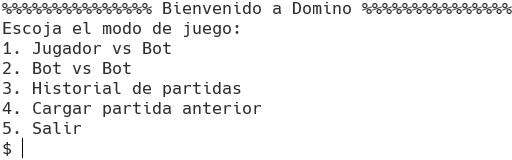
\includegraphics[]{pf1.png}
    \caption{Menu de opciones de juego}
  \end{figure}

  En caso de que se seleccione la opcion 1 se pide el nombre del jugador y se luego se pregunta si se quiere guardar la configuracion de la partida. En caso de que se seleccione la opcion 2 se inicia una partida entre dos bots. En caso de que se seleccione la opcion 3 se muestra el historial de partidas guardadas. En caso de que se seleccione la opcion 4 se muestra la lista de archivos de configuracion disponibles.

  \begin{figure}[h!]
    \centering
    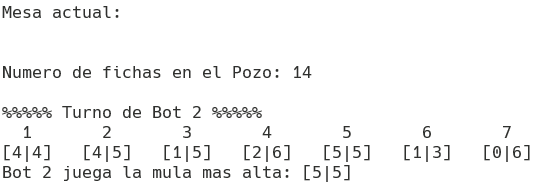
\includegraphics[]{pf2.png}
    \caption{Ingresar nombre de jugador y guardar configuracion}
  \end{figure}

  Al iniciar una partida se muestra la mesa, el pozo y las fichas del jugador. En caso de que sea el primer turno del jugador tira automaticamente la mula más alta o la ficha más alta. 

  \begin{figure}[h!]
    \centering
    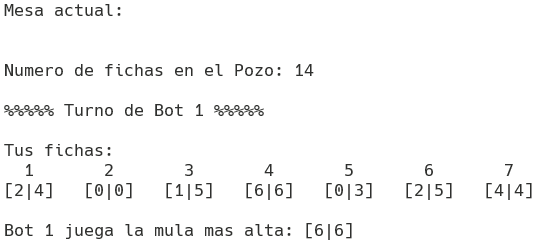
\includegraphics{pf3.png}
    \caption{Inicio del juego}
  \end{figure}
  
  Los siguientes turnos son diferentes dependiendo del tipo de jugador. En caso de que sea un bot se espera 3 segundos antes de que juegue su ficha. En caso de que sea una persona se le pide que seleccione la ficha que quiere jugar y el lado donde la quiere jugar.

  \begin{figure}[h!]
    \centering 
    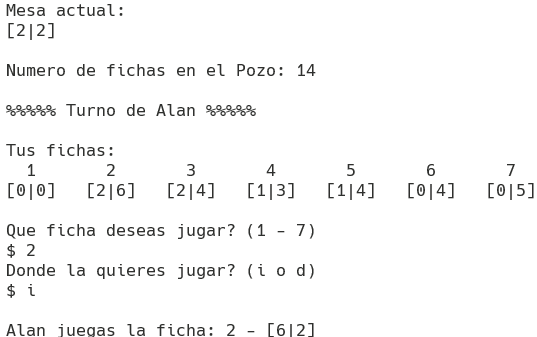
\includegraphics{pf4.png}
    \caption{Turno de jugador Persona}
  \end{figure}

  \begin{figure}[h!]
    \centering
    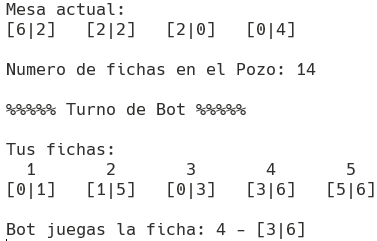
\includegraphics{pf5.png}
    \caption{Turno de jugador Bot}
  \end{figure}
  
  En caso de que un jugador necesite robar una ficha se muestra un mensaje indicandolo y se vuelven a imprimir sus fichas.

  \begin{figure}[h!]
    \centering
    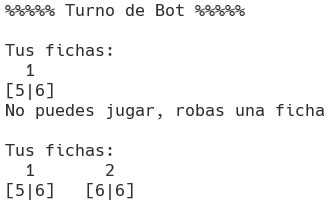
\includegraphics{pf6.png}
    \caption{Mensaje de robar ficha} 
  \end{figure}

  Al ganar el jugador se muestra un mensaje de victoria y se termina el programa.

  \begin{figure}[h!]
    \centering
    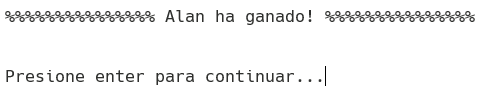
\includegraphics[]{pf7.png}
    \caption{Mensaje de victoria}
  \end{figure}

  Al abrir el historial de partidas se muestra una tabla con el nombre del ganador, el turno en el que gano y la fecha en la que se jugo la partida.

  \begin{figure}[h!]
    \centering
    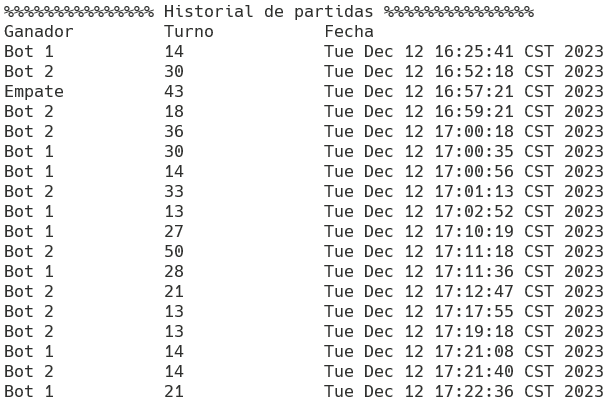
\includegraphics[]{pf8.png}
    \caption{Historial de partidas}
  \end{figure}

  Si se quiere cargar una partida guardada se muestra la lista de archivos de configuracion disponibles y se pide que se seleccione el archivo de configuracion que se quiere cargar.

  \begin{figure}[h!]
    \centering
    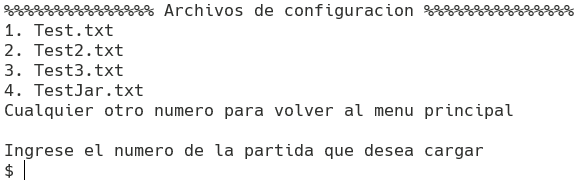
\includegraphics[]{pf9.png}
    \caption{Lista de archivos de configuracion}
  \end{figure}

  \subsection{Documentacion de JavaDoc}
  Al ejecutar el comando \textit{javadoc -d documentacion domino/*.java} se genera la documentacion de JavaDoc en la carpeta \textit{documentacion}. Algunos ejemplos de la documentacion generada se muestran a continuación y lo restante se encuentra en la dirección \url{https://dominov2.netlify.app}.

  \begin{figure}[h!]
    \centering
    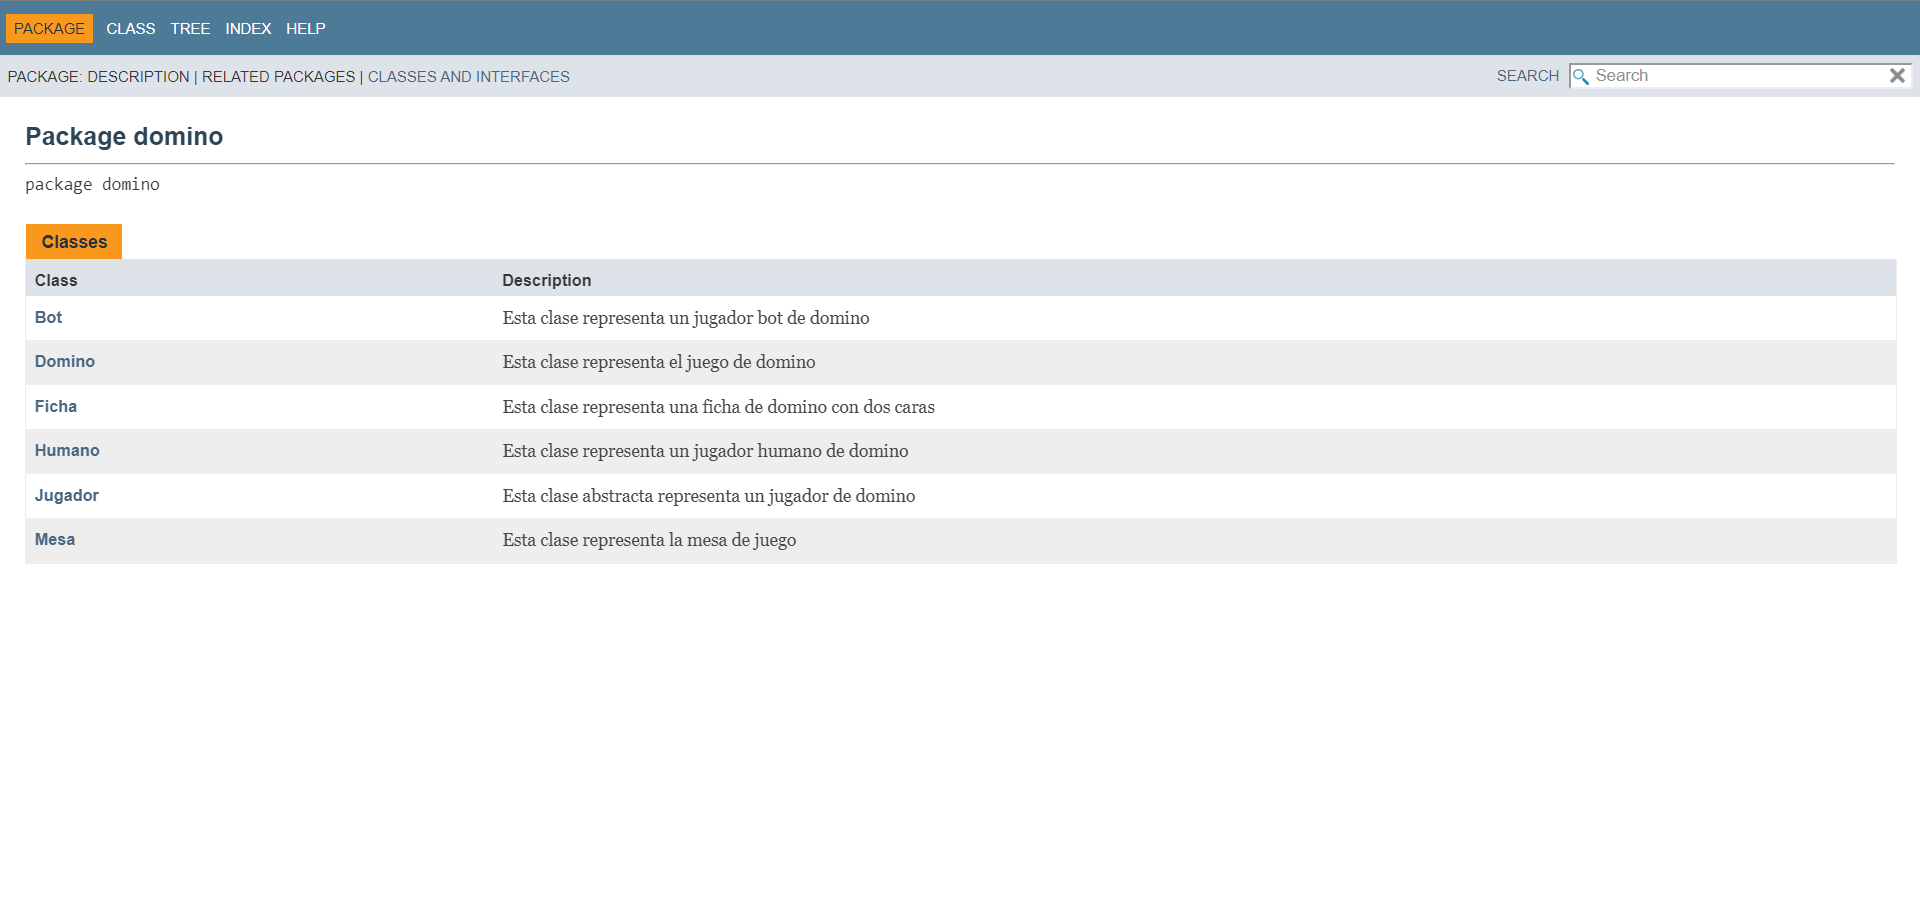
\includegraphics[width=\textwidth]{doc1.png}
    \caption{Página principal}
  \end{figure}

  \begin{figure}[h!]
    \centering
    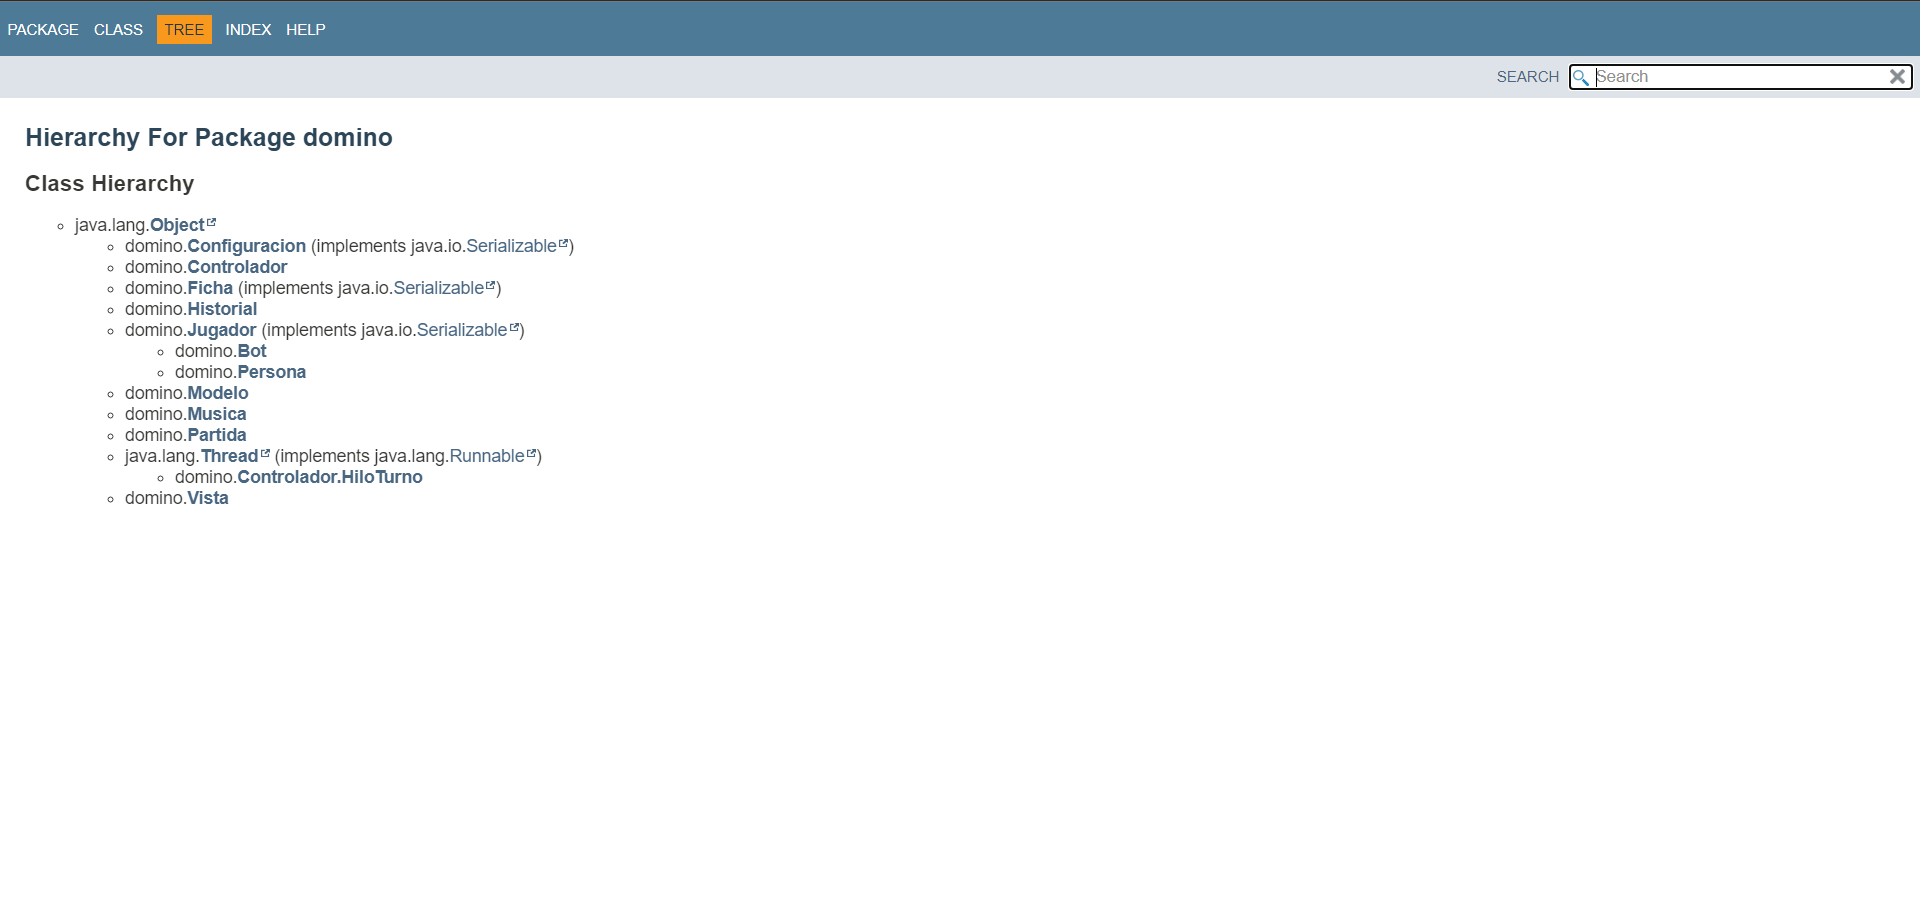
\includegraphics[width=\textwidth]{doc2.png}
    \caption{Árbol de jerarquia de clases}
  \end{figure}

  \begin{figure}[h!]
    \centering
    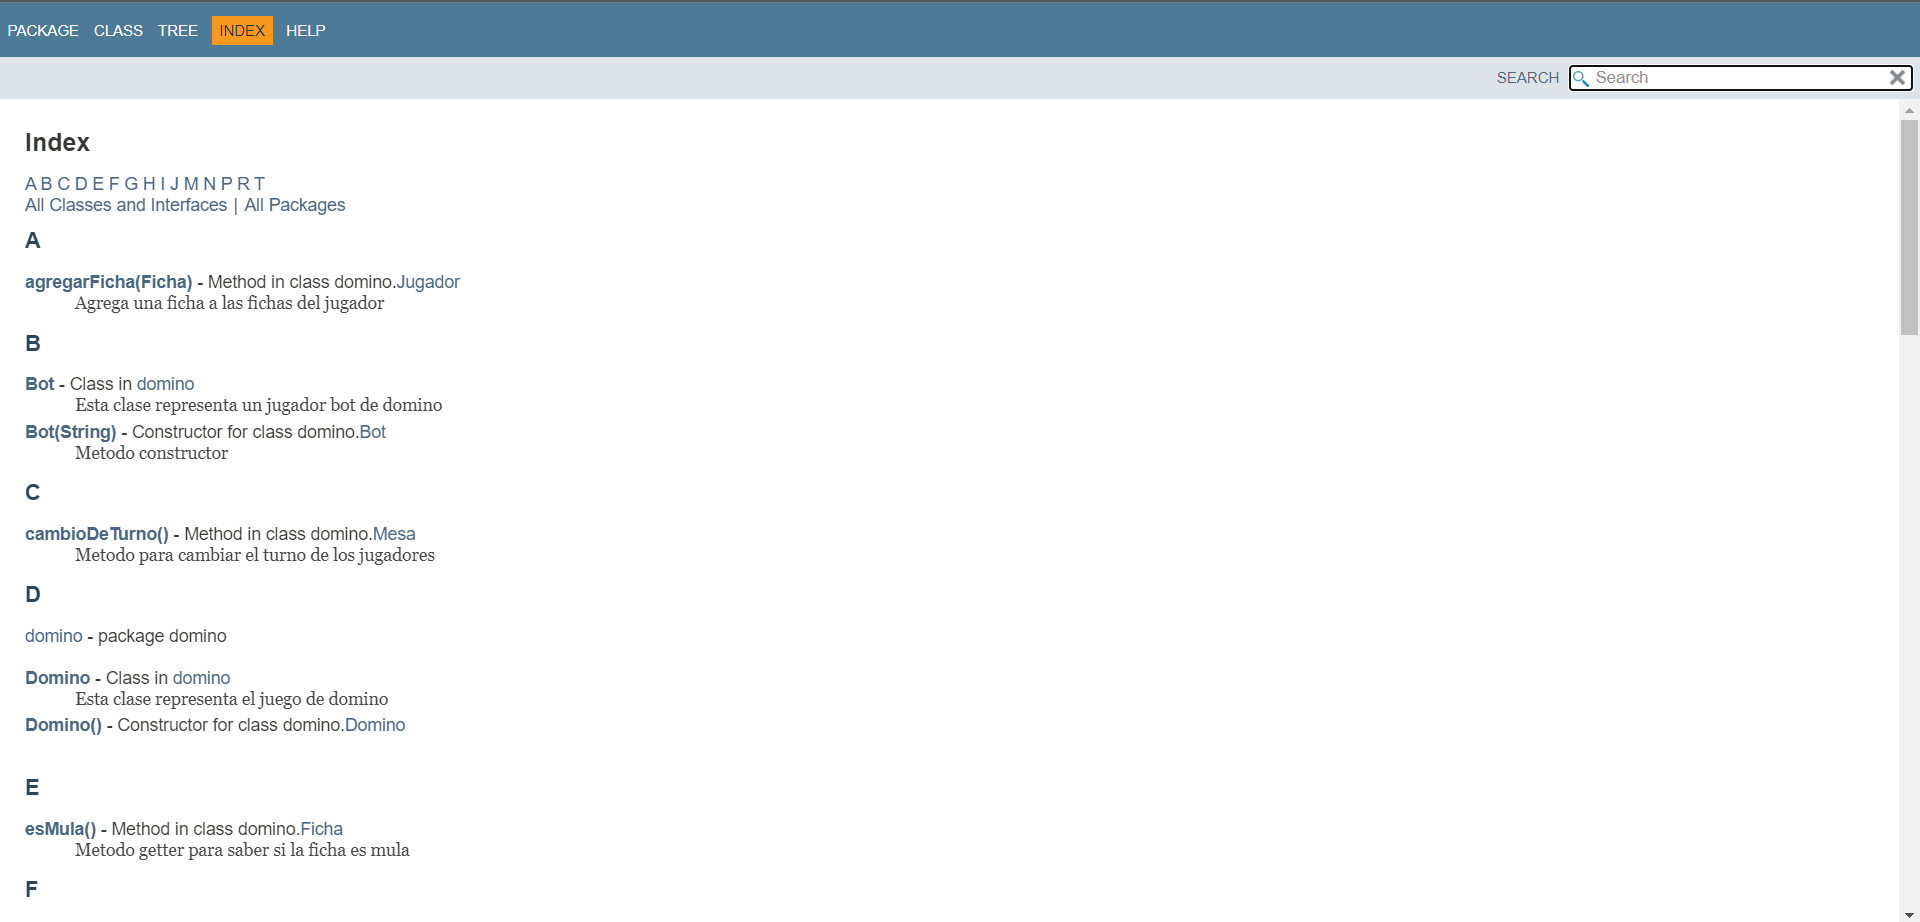
\includegraphics[width=\textwidth]{doc3.png}
    \caption{Índice alfabetico}
  \end{figure}

  \begin{figure}[h!]
    \centering
    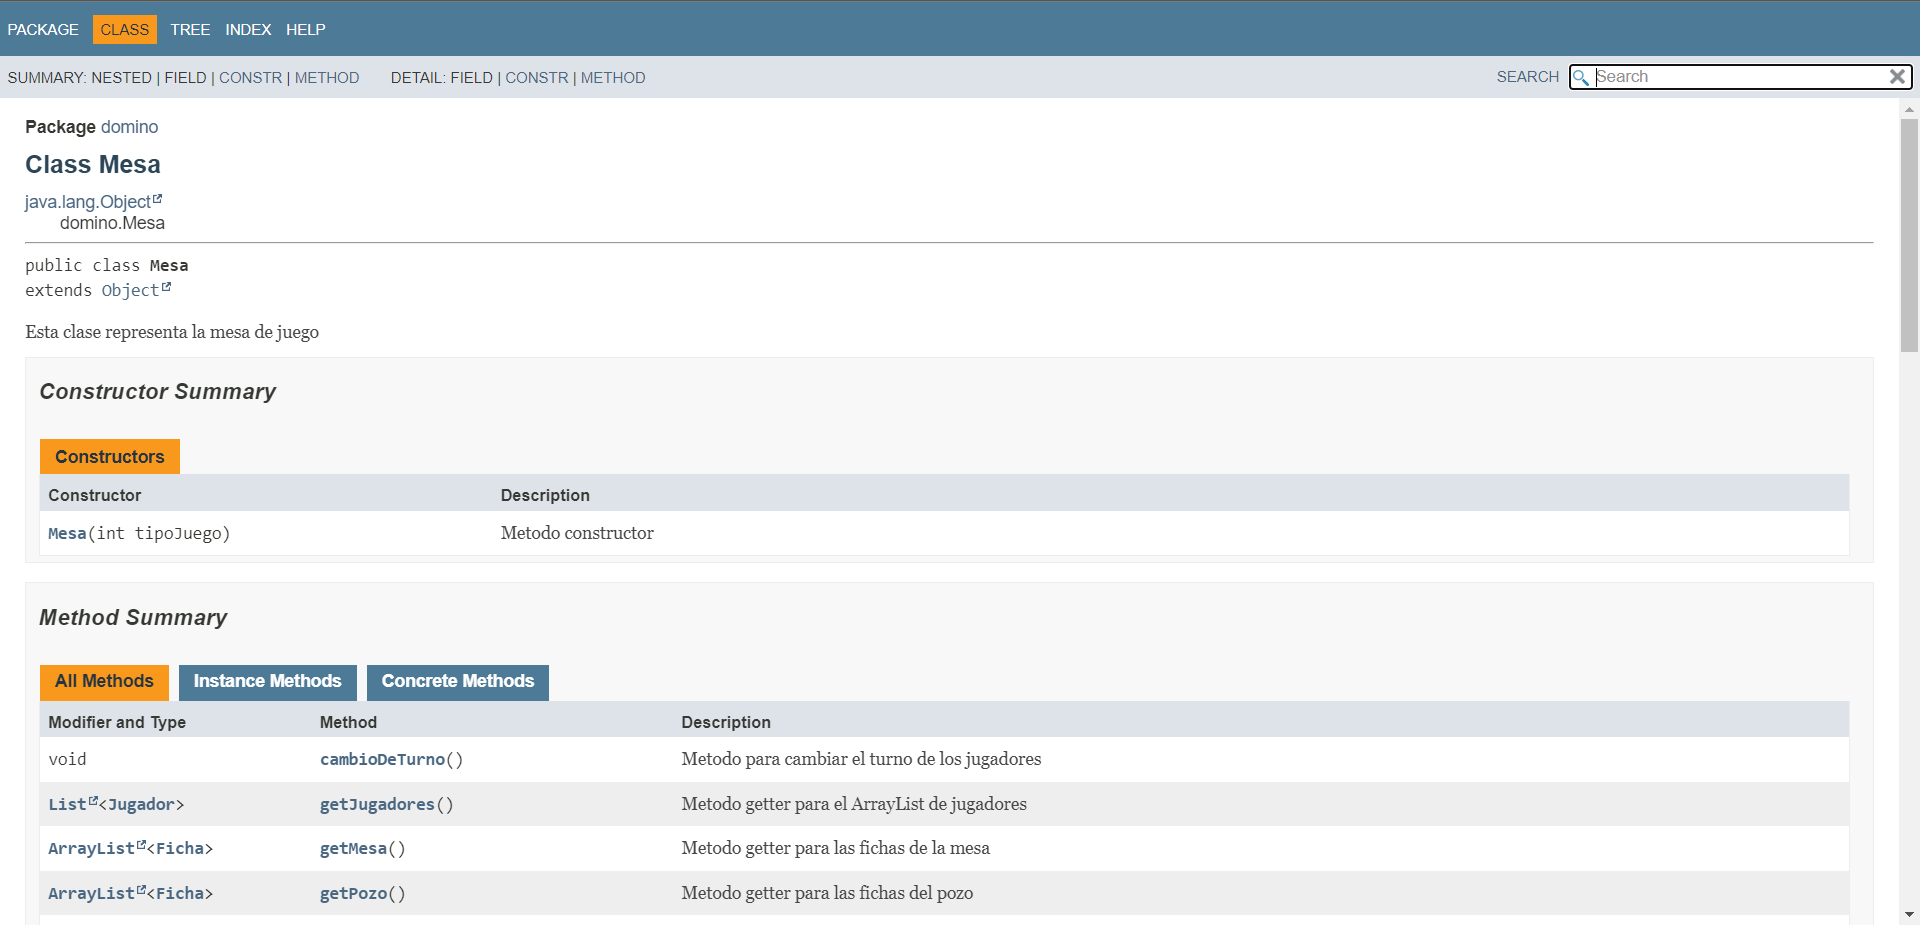
\includegraphics[width=\textwidth]{doc4.png}
    \caption{Página de la clase \textit{Controlador}} 
  \end{figure}
\end{document}